\documentclass[10pt,twocolumn,letterpaper]{article}

\usepackage{cvpr}
\usepackage{times}
\usepackage{epsfig}
\usepackage{graphicx}
\usepackage{amsmath}
\usepackage{amssymb}

\usepackage[utf8]{inputenc}
\usepackage{listings}
\usepackage{float}
\usepackage{graphics}
\usepackage{graphicx} 
\usepackage{caption} 
\usepackage{subcaption} 
\usepackage{verbatim}
\usepackage{cite}

% Include other packages here, before hyperref.

% If you comment hyperref and then uncomment it, you should delete
% egpaper.aux before re-running latex.  (Or just hit 'q' on the first latex
% run, let it finish, and you should be clear).
\usepackage[pagebackref=true,breaklinks=true,letterpaper=true,colorlinks,bookmarks=false]{hyperref}

\cvprfinalcopy % *** Uncomment this line for the final submission

\def\cvprPaperID{****} % *** Enter the CVPR Paper ID here
\def\httilde{\mbox{\tt\raisebox{-.5ex}{\symbol{126}}}}

% Pages are numbered in submission mode, and unnumbered in camera-ready
\ifcvprfinal\pagestyle{empty}\fi
\begin{document}
%%%%%%%%% TITLE
\title{Experiments in Deferred Shading for Training Image Classifiers}

\author{Kristofer Schlachter\\
NYU\\
{\tt\small schlacht@cims.nyu.edu}
% For a paper whose authors are all at the same institution,
% omit the following lines up until the closing ``}''.
% Additional authors and addresses can be added with ``\and'',
% just like the second author.
% To save space, use either the email address or home page, not both
\and
Connor DeFanti\\
NYU\\
{\tt\small defanti@cims.nyu.edu}
\and
Ken Perlin\\
NYU\\
{\tt\small perlin@nyu.edu}
\and
Jonathan Tompson\\
Google Brain\\
{\tt\small tompson@google.com}
}

\maketitle
%\thispagestyle{empty}
\maketitle

%%%%%%%%%%%%%%%%%%%%%%%%%%%%%%%%%%%%%%%%%%%%%%%%%%%%%%%%%%%%%%%%%%%%%%%%%%%%%%%%%%%%%%%%%%%%%%%%%%%%%%%%%%%%
%%%%%%%%%%%%%%%%%%%%%%%%%%%%%%%%%%%%%%%%%%%%%%%%%%%%%%%%%%%%%%%%%%%%%%%%%%%%%%%%%%%%%%%%%%%%%%%%%%%%%%%%%%%%
\section{Abstract}
%%%%%%%%%%%%%%%%%%%%%%%%%%%%%%%%%%%%%%%%%%%%%%%%%%%%%%%%%%%%%%%%%%%%%%%%%%%%%%%%%%%%%%%%%%%%%%%%%%%%%%%%%%%%
%%%%%%%%%%%%%%%%%%%%%%%%%%%%%%%%%%%%%%%%%%%%%%%%%%%%%%%%%%%%%%%%%%%%%%%%%%%%%%%%%%%%%%%%%%%%%%%%%%%%%%%%%%%%

As synthetic imagery is used more frequently in training deep models, it is important to understand how different synthesis techniques impact the performance of models.  We measure the effectiveness of several different synthesis techniques relative to one another as well as to the real data that they seek to replicate.  We also introduce learned synthesis techniques that better train models than the most realistic graphical methods used by standard rendering packages or approach their fidelity using far less computation.  We accomplish this by learning shading of geometry as well as denoising the results of low sample Monte Carlo image synthesis.  Our major contributions are (i) a dataset that allows comparison of real and synthetic versions of the same scene, (ii) an augmented data representation that boosts the stability of learning and improves the datasets accuracy, and (iii) three different partially differentiable rendering techniques where lighting, denoising and shading are learned. We improve a state of the art generative adversarial network architecture to generate datasets that approach the performance of the full global illumination rendering and approach the performance of training on real data.
%%%%%%%%%%%%%%%%%%%%%%%%%%%%%%%%%%%%%%%%%%%%%%%%%%%%%%%%%%%%%%%%%%%%%%%%%%%%%%%%%%%%%%%%%%%%%%%%%%%%%%%%%%%%
%%%%%%%%%%%%%%%%%%%%%%%%%%%%%%%%%%%%%%%%%%%%%%%%%%%%%%%%%%%%%%%%%%%%%%%%%%%%%%%%%%%%%%%%%%%%%%%%%%%%%%%%%%%%
\section{Introduction - Paper's Contribution}
%%%%%%%%%%%%%%%%%%%%%%%%%%%%%%%%%%%%%%%%%%%%%%%%%%%%%%%%%%%%%%%%%%%%%%%%%%%%%%%%%%%%%%%%%%%%%%%%%%%%%%%%%%%%
%%%%%%%%%%%%%%%%%%%%%%%%%%%%%%%%%%%%%%%%%%%%%%%%%%%%%%%%%%%%%%%%%%%%%%%%%%%%%%%%%%%%%%%%%%%%%%%%%%%%%%%%%%%%

Deep learning commonly requires large labeled datasets \cite{imagenet}, \cite{coco}, which can be time consuming, expensive or impractical to collect.  As a result, more and more synthetic data has been used to overcome these issues in dataset creation \cite{DBLP:journals/corr/RichterVRK16} \cite{DBLP:journals/corr/ShafaeiLS16} \cite{DBLP:journals/corr/ZhangSYSLJF16} \cite{DBLP:journals/corr/SixtWL17}. However, using synthetic data can introduce problems that arise from the differences in the distributions of the real and synthesized data \cite{2014arXiv1409.7495G}.  Usually the best way to reduce the differences is to use the most realistic simulation method for synthesizing images, in this case a Global Illumination (GI) based renderer.  Unfortunately, the computational cost of most GI renderers can be prohibitive.  Recently, there has been research into boosting the effectiveness of existing synthetic data\cite{DBLP:journals/corr/ShrivastavaPTSW16}.  However, these new techniques were not benchmarked against using real data or against other rendering techniques.

This work explores the effectiveness of various rendering methods which range from very low to very high computational cost.   Furthermore, not only do we compare the performance among the synthetic techniques, but we also compare against using real data.  We can do this because we extend an existing dataset by rendering each scene to a Geometry Buffer (g-buffer),  \footnote{A g-buffer is the first step in a two step process called deferred shading. The second step is the actual shading of the geometry stored in the g-buffer.} which gives us a standard set of 3D scenes where geometric transformations are frozen in place.

%which is a rendering of a scene that freezes the objects in the scene and puts the 3D information describing the scene from a given state of the camera, geometry and materials into a set of buffers.  You can then use those g-buffers that correspond to the original dataset and shade them in a separate step. 
%This two step process of rendering geometry and material information to a g-buffer and then in second step shading the scene to produce the final image is called deferred shading.  

%By using a g-buffer, we have isolated the physical process of shading a surface from the geometric process of geometry pose and projection.  The shading process is also isolated from camera parameters including location, orientation and field of view. This allowed us to directly compare different rendering methods and enabled us to isolate any performance difference due to shading alone.

Capitalizing on this standard 3D scene representation we setup a number of experiments to compare rendering methods of increasing sophistication and computational cost.  We then measure the benefit of adding certain rendering techniques and see if the computational cost can be justified.  These experiments revealed which image features are important and which are not.  We use a full GI 128 sample rendering as the method whose performance we sought to match or surpass.  We are able to do this by using non-standard rendering techniques that involve using convolutional neural nets to learn shading functions.  This is a form of differentiable rendering where the shading is differentiable. We used learned shading to denoise low sample count GI rendering and compared it to high sample count images.  We also explored the refining technique in \cite{DBLP:journals/corr/ShrivastavaPTSW16},  and we extend it to use g-buffers and other performance enhancing modifications.

\subsection{Contributions}
\begin{enumerate}
\item We provide a dataset that allows the direct comparison of training on real data versus synthetic by including 3D scans of the objects that are in the photographic dataset.
\item We create multiple partially differentiable renderers that can learn shading functions.
\item We a method of using GAN trained generative models in a novel way to create an augmented dataset.
\item We contribute a thorough comparison of the performance of all the rendering methods with real data.
\end{enumerate}
%%%%%%%%%%%%%%%%%%%%%%%%%%%%%%%%%%%%%%%%%%%%%%%%%%%%%%%%%%%%%%%%%%%%%%%%%%%%%%%%%%%%%%%%%%%%%%%%%%%%%%%%%%%%
%%%%%%%%%%%%%%%%%%%%%%%%%%%%%%%%%%%%%%%%%%%%%%%%%%%%%%%%%%%%%%%%%%%%%%%%%%%%%%%%%%%%%%%%%%%%%%%%%%%%%%%%%%%%
\section{Related Work}
%%%%%%%%%%%%%%%%%%%%%%%%%%%%%%%%%%%%%%%%%%%%%%%%%%%%%%%%%%%%%%%%%%%%%%%%%%%%%%%%%%%%%%%%%%%%%%%%%%%%%%%%%%%%
%%%%%%%%%%%%%%%%%%%%%%%%%%%%%%%%%%%%%%%%%%%%%%%%%%%%%%%%%%%%%%%%%%%%%%%%%%%%%%%%%%%%%%%%%%%%%%%%%%%%%%%%%%%%

There are many ways to generate images and more than one technique is used in this paper, including using g-buffers as input.  Previous papers have used a g-buffers to learn a shading techniques.  Nalbach \textit{et al.} \cite{DBLP:journals/corr/NalbachAMSR16} uses a similar model architecture as the denoiser we employ as well as using a g-buffer as input.  The authors use it to learn to approximate screen space shading techniques with a data-driven approach, to see if data driven methods can replicate the standard shading methods used in games.  They also use the Structured Similarity (SSIM) loss which is used in our work. 
%Loss Functions for Neural Networks for Image Processing 
Zhao \textit{et al.} \cite{DBLP:journals/corr/ZhaoGFK15} discusses the motivation of using Structured Similarity (SSIM) as a loss function for image generators.

%In SimGAN they use data and 4x data.  What they mean is 1/4 of the dataset vs the whole dataset. Which is not the same as creating more novel data from GANs.\\



There have been recent advances in denoising low sample count images calculated by Global Illumination (GI) based renderers.
%Spatiotemporal Variance-Guided Filtering: Real-Time Reconstruction for Path-Traced Global Illumination 
Shied \textit{et al.} \cite{Schied:2017:SVF:3105762.3105770} denoises low sample count GI images by combining neighboring frames and feeding them into a fixed spatiotemporal filter.  The authors emphasis is on temporal stability , efficient computation and denoising single sample frames in real-time. Their authors do not employ machine learning in their method. 
%Interactive Reconstruction of Monte Carlo Image Sequences using a Recurrent Denoising Autoencoder 
Chaitanya \textit{et al} \cite{Chaitanya:2017:IRM:3072959.3073601} along with 
%Kernel-Predicting Convolutional Networks for Denoising Monte Carlo Renderings 
Bako \textit{et al.} \cite{Bako17} and 
%A Machine Learning Approach for Filtering Monte Carlo Noise
Kalantari \textit{et al.} \cite{Kalantari:2015:MLA:2809654.2766977} all use machine learning to denoise Monte Carlo (GI) renderings.  Our work uses a modified form of the model presented in \cite{Chaitanya:2017:IRM:3072959.3073601}.

Further use of global illumination for training classifiers has been explored.
%Physically-Based Rendering for Indoor Scene Understanding Using Convolutional Neural Networks 
Zhang \textit{et al.} \cite{DBLP:journals/corr/ZhangSYSLJF16} use a custom created large 3D indoor dataset to conduct experiments relating the performance of different renderers and lighting for various machine learning tasks. They learn normal estimation, semantic segmentation, and object boundary detection.  They use two types of rendering, a rasterization renderer using OpenGL with direct lighting and what they call "local lighting." Local lighting, as described in their paper, is placing many lights into the environment but only use the closest 8 lights for direct lighting computation.  Both OpenGL methods do not include any GI or shadowing. They have two lighting conditions for their GI based rendering,  indirect light coming from through windows and local light coming from emissive objects within the scene.  They compare their results with a real dataset and use the real dataset to fine-tune their training. The only conclusions they can draw from their experiments are that more realistic data is better and that using a GI based renderer provides the results for synthetic data.


%Model-driven Simulations for Deep Convolutional Neural Networks 
Veeravasarapu \textit{et al.} \cite{DBLP:journals/corr/VeeravasarapuRR16} discuss Monte Carlo methods for generating synthetic data, and examine several different simulated datasets. They tested various different levels of fidelity (measured in samples-per-pixel) and concluded that beyond a certain threshold (40 spp for their specific scenes), increases in rendering fidelity do not increase the data training accuracy.

% How useful is photo-realistic rendering for visual learning? 
Movshovitz-Attias \textit{et al.} \cite{DBLP:journals/corr/Movshovitz-Attias16} tested synthetic data for training combined with real data for viewpoint estimation. The paper demonstrated that synthetic data produced by a high-quality renderer and added to a real dataset can produce training accuracies that are competitive with natural (real) data. Their work focused on rendering parameters, such as lighting positions, background, and camera shutter speed. They accounted for any performance shortfall in their synthetic data versus real as due to the difference between the domains in their datasets.  We designed our dataset so you could not use that argument. The part of the rendering process that they varied was the material which is something we hold constant. This makes their work complementary due to our focus on light interaction and propagation.

%Playing for Data: Ground Truth from Computer Games
%Play and Learn: Using Video Games to Train Computer Vision Model 
Using a video game engine for dataset creation has been explored by Richter \textit{et al.} \cite{DBLP:journals/corr/RichterVRK16} and  Shafaei \textit{et al.} \cite{DBLP:journals/corr/ShafaeiLS16}. They explored the use of video game snapshots to show that it could train image segmentation models. While we sought to answer the question of classification over segmentation, this paper did provide interesting insights into the use of data that was rendered at real time for computer vision training problems.

%Conditional Image Synthesis with Auxiliary Classifier GANs \cite{DBLP:journals/corr/OdenaOS16} uses label data to improve the results of GANs.  They also use SSIM as a way to measure their results which we attempt to do as well.

%Generative Image Modeling using Style and Structure Adversarial Networks 
To learn shading, we used Generative Adversarial Networks(GAN) which were first introduced by Goodfellow \textit{et al.} \cite{goodfellow}. Since then many works have used them to synthesize images. Wang and Gupta \cite{DBLP:journals/corr/WangG16} used multiple GANs for unsupervised learning on real data, separating structure and style of the image data into two separate GANs and later recombining the results. This method was applied to data retrieval for images and classification performance was not measured.

%Learning from Simulated and Unsupervised Images through Adversarial Training 
A GAN based method that uses unlabeled data to refine realistic rendered images was pioneered by
Shrivastava \textit{et al.} \cite{DBLP:journals/corr/ShrivastavaPTSW16}. The paper describes an architecture that takes in rendered images and makes them more realistic by using an adversarial loss to tune a refiner model that transforms the pixels enough to fool a discriminator.  An issue with their method is that they don't have a principled way of telling when to stop the learning of a refiner and thus require a human to decide that an image ``looks real.''  A problem with using their approach is that what might be most realistic to a human may not maximize the utility in training a classifier. We use this paper as a starting point for our GAN experiments,  but we address the difficulty of comparing a methods effectiveness against other rendering techniques as well as real data.  We also address the method of choosing the best GAN to use for the final refiner.  

%RenderGAN: Generating Realistic Labeled Data 
Having a partially differentiable renderer has been explored by Sixt \textit{et al.} \cite{DBLP:journals/corr/SixtWL17}. In their paper they train a differentiable 3D renderer, except their model is scene and application specific. Their model is restricted to learning a rendering of a specific single geometric tag that can be approximated by a circle. This can be done because geometric transformations seem to happen in plane and can be thought of as 2D.  Also, their lighting is approximated by a 2D gradient, and they learn hand picked application-specific features such as blurriness, background and detail.  In the end their methods are narrowly applicable to the images they are trying to approximate and do not generalize to a full 3D renderer. \\

%Unsupervised Domain Adaptation by Backpropagation 
%Domain adaptation without modifying the dataset itself is discussed by Ganin and Lempitsky \cite{2014arXiv1409.7495G} who modify the gradients of a classifier during learning in order to make the learned model domain invariant.  

%Generative Adversarial Nets \cite{2014arXiv1406.2661G}\\
%Learning Methods for Generic Object Recognition with Invariance to Pose and Lighting \cite{LeCun:2004:LMG:1896300.1896315}\\


%%%%%%%%%%%%%%%%%%%%%%%%%%%%%%%%%%%%%%%%%%%%%%%%%%%%%%%%%%%%%%%%%%%%%%%%%%%%%%%%%%%%%%%%%%%%%%%%%%%%%%%%%%%%
\subsection{Graphics and Rendering Background}
%%%%%%%%%%%%%%%%%%%%%%%%%%%%%%%%%%%%%%%%%%%%%%%%%%%%%%%%%%%%%%%%%%%%%%%%%%%%%%%%%%%%%%%%%%%%%%%%%%%%%%%%%%%%

In our experiments, we use some rendering techniques that require some background.  The first is a geometry buffer (G-Buffer).
%%%%%%%%%%%%%%%%%%%%%%%%%%%%%%%%%%%%%%%%%%%%%%%%%%%%%%%%%%%%%%%%%%%%%%%%%%%%%%%%%%%%%%%%%%%%%%%%%%%%%%%%%%%%
\subsubsection{G-Buffer}
%%%%%%%%%%%%%%%%%%%%%%%%%%%%%%%%%%%%%%%%%%%%%%%%%%%%%%%%%%%%%%%%%%%%%%%%%%%%%%%%%%%%%%%%%%%%%%%%%%%%%%%%%%%%

In real-time rendering, a popular way to draw images is to store the rasterized geometry information into a set of images or buffers called a G-Buffer \cite{Saito:1990:CRS:97879.97901}, which is short for geometry buffer. 

G-Buffers separate the geometric processes such as transformation, projection and depth testing, from physical processes such as shading and texture mapping.  This is accomplished by the buffers accumulating the geometry information in the first pass and then lighting each pixel of the output on a second pass.  This is in comparison to a forward renderer which calculates geometry information and performs lighting and shadowing in one pass, followed by and writing the result to the output buffer.  
%The inefficiency that the G-Buffer addresses is that the information can then be replaced by an object that is drawn later in the stream.  Pixels can be overdrawn many many times which can cause a lot of wasted lighting computation. 
G-Buffers allow for ``deferred shading,'' where expensive lighting and shadowing computation is done after all of the visible geometry is encoded into its buffers.\\

The encoding of our geometry state into G-Buffers allows for simplified testing of different shading techniques on the identical 3D scenes.
In our experiments, our G-Buffer consists of the scene encoded geometry normals, geometry diffuse color (also referred to as albedo), and the linear depth from the camera to the visible geometry.  See figures \ref{fig:GBUFFER_ALBEDO}, \ref{fig:GBUFFER_NORMALS}, and \ref{fig:GBUFFER_DEPTH} for examples.
\begin{figure}[h!]
\centering
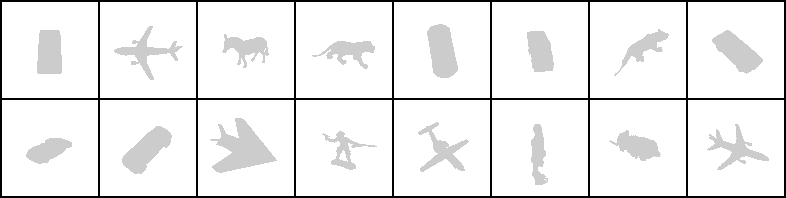
\includegraphics[width=0.8\columnwidth]{./assets/synth_albedo.jpg}
\caption{Albedo Map}
\label{fig:GBUFFER_ALBEDO}
\end{figure}

%\begin{figure}[h!]
%\centering
%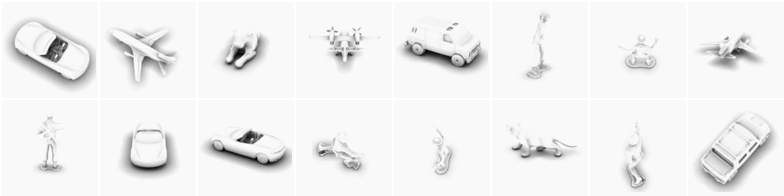
\includegraphics[width=0.8\textwidth]{./assets/ao_sample.png}
%\caption{Occlusion Map}
%\label{fig:GBUFFER_SHADOW}
%\end{figure}

\begin{figure}[h!]
\centering
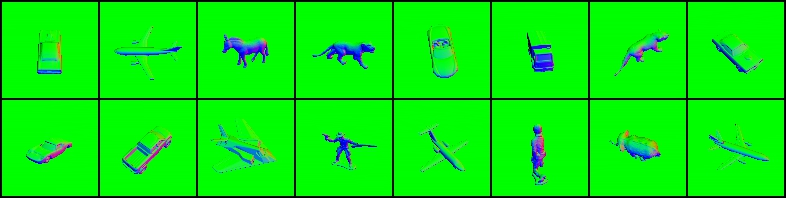
\includegraphics[width=1.0\columnwidth]{./assets/synth_world_normals.jpg}
\caption{World Space Normals Map in RGB}
\label{fig:GBUFFER_NORMALS}
\end{figure}

\begin{figure}[h!]
\centering
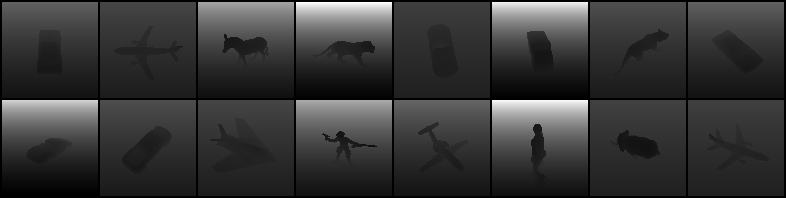
\includegraphics[width=1.0\columnwidth]{./assets/synth_linear_depth.jpg}
\caption{Depth Map}
\label{fig:GBUFFER_DEPTH}
\end{figure}

%%%%%%%%%%%%%%%%%%%%%%%%%%%%%%%%%%%%%%%%%%%%%%%%%%%%%%%%%%%%%%%%%%%%%%%%%%%%%%%%%%%%%%%%%%%%%%%%%%%%%%%%%%%%
\subsubsection{Spherical Harmonics}
%%%%%%%%%%%%%%%%%%%%%%%%%%%%%%%%%%%%%%%%%%%%%%%%%%%%%%%%%%%%%%%%%%%%%%%%%%%%%%%%%%%%%%%%%%%%%%%%%%%%%%%%%%%%
\begin{figure}[h!]
\centering
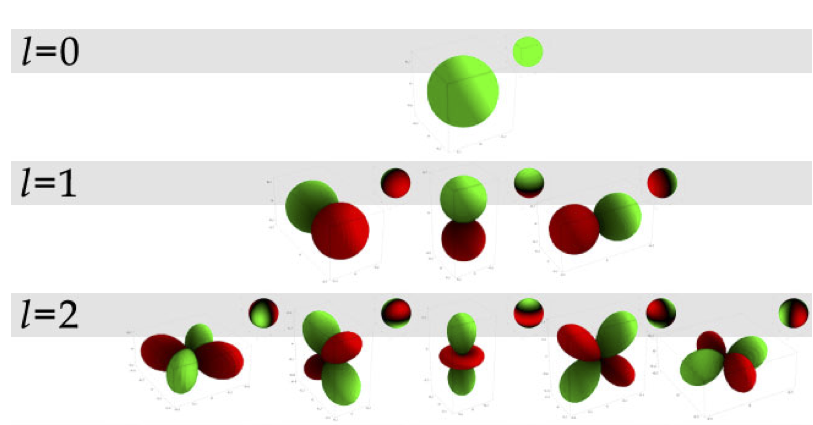
\includegraphics[width=1.0\columnwidth]{./assets/SHBands.png}
\caption{Visualization of first 3 bands of the spherical harmonics functions. ``Plotted as unsigned spherical functions by distance from the origin and by color on unit sphere. Green are positive values and red are negative.'' \cite{G03}  These are the corresponding 9 functions to the 9 coefficients we learn for lighting.}
\label{fig:SHBands01}
\end{figure}
\begin{figure}[h!]
\centering
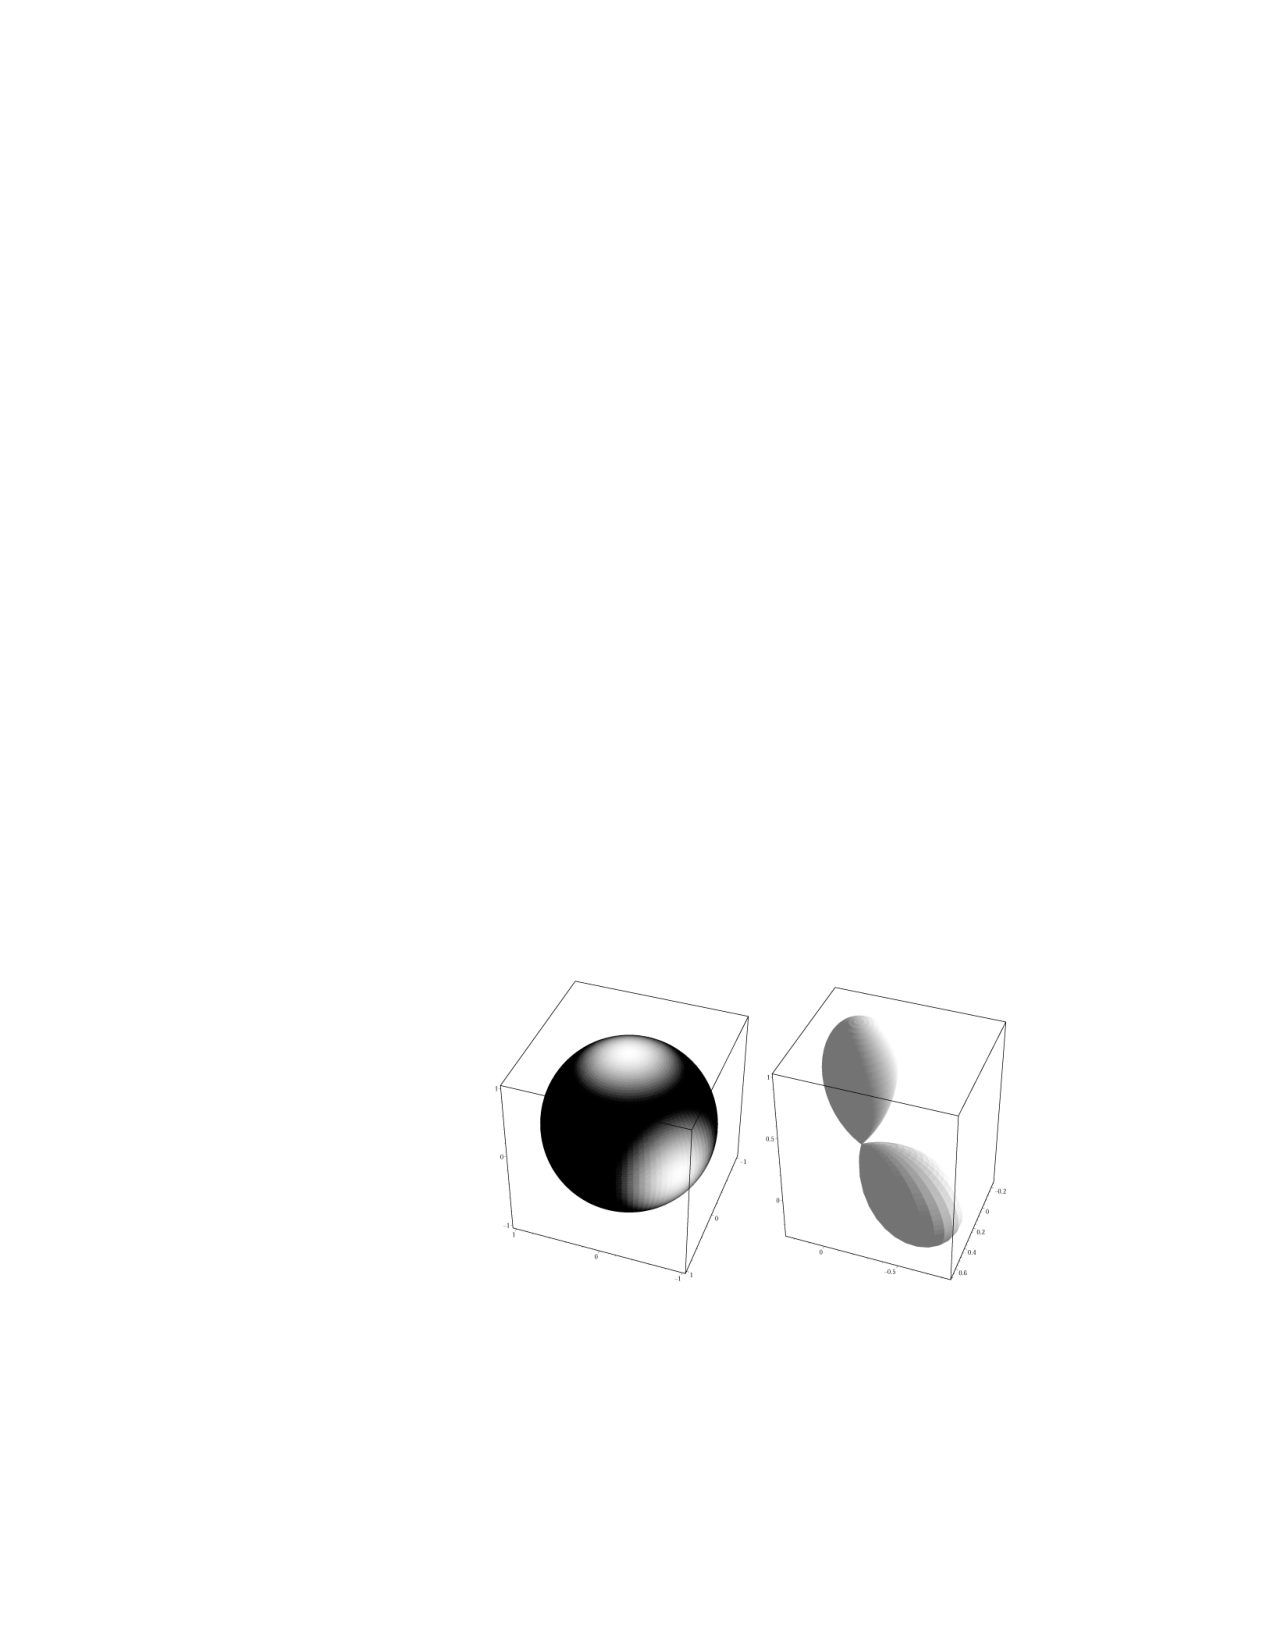
\includegraphics[width=0.8\columnwidth]{./assets/SHOneBandNoCaption.pdf}
\caption{Visualization of lighting function using [RIGHT] a lit sphere  and [LEFT] lobes. \cite{G03}}
\label{fig:SHBands02}
\end{figure}
In our experiments, we also use a set of functions called Spherical Harmonics (SH) to learn the lighting in the environment. Spherical harmonics are a set of functions that approximate an arbitrary spherical function, such as the distribution of incoming or outgoing light \cite{Ramamoorthi:2001:ERI:383259.383317}.  They are continuous and rotationally invariant. They are grouped into levels, where each level is a set of orthogonal functions of finer detail, resolution, or frequency \cite{Shreiner:2013:OPG:2544032}.  To represent the smooth lighting in our experiments, we only need the first three levels which are a constant, linear polynomials, and quadratic polynomials of the surface normal.\\

See Figure \ref{fig:SHBands01} for a visualization of the first three levels and see Figure \ref{fig:SHBands02} to see a visualization of a diffuse lighting function.\\

An advantage to using spherical harmonics for lighting is that you can represent a smooth lighting environment with just 9 floats.  This allows us to parameterize a lighting function with far fewer parameters compared to other representations\footnote{Image Based Lighting for instance.  It requires 6 images!}. This has the effect of drastically reducing the search space when trying to learn a parameterized lighting.

%%%%%%%%%%%%%%%%%%%%%%%%%%%%%%%%%%%%%%%%%%%%%%%%%%%%%%%%%%%%%%%%%%%%%%%%%%%%%%%%%%%%%%%%%%%%%%%%%%%%%%%%%%%%
\subsubsection{Spherical Harmonics Network}
%%%%%%%%%%%%%%%%%%%%%%%%%%%%%%%%%%%%%%%%%%%%%%%%%%%%%%%%%%%%%%%%%%%%%%%%%%%%%%%%%%%%%%%%%%%%%%%%%%%%%%%%%%%%

We used this representational advantage in our experiments by creating a pyTorch \cite{PYTORCH} module that calculates three levels of the spherical harmonics basis functions.  These functions were parameterized by 9 floats.  The input to the network is the surface normal at every pixel, which is conveniently stored in the normal buffer part of the g-buffer. The normal buffer is input into the SH module which outputs a shaded image that can be composited with shadowing and albedo.

%%%%%%%%%%%%%%%%%%%%%%%%%%%%%%%%%%%%%%%%%%%%%%%%%%%%%%%%%%%%%%%%%%%%%%%%%%%%%%%%%%%%%%%%%%%%%%%%%%%%%%%%%%%%
\subsubsection{Ambient Occlusion}
%%%%%%%%%%%%%%%%%%%%%%%%%%%%%%%%%%%%%%%%%%%%%%%%%%%%%%%%%%%%%%%%%%%%%%%%%%%%%%%%%%%%%%%%%%%%%%%%%%%%%%%%%%%%

Given that we are only allowing smoothly changing lighting, there is a very simple first order approximation to global illumination that can approximate it. It is called Ambient Occlusion and it is considered a form of global illumination because it takes into account the geometry in the scene\cite{Miller:1994:EAL:192161.192244}.  For each point on the surface of the scene geometry, it approximates how exposed it is to incoming ambient light sources.  It does this by calculating how much of the hemisphere around that point is blocked by nearby surfaces. For lighting conditions is close to a uniformly bright hemisphere, like an overcast day, then ambient occlusion is a good approximation of global illumination\footnote{See Figure~\ref{fig:AO1} to see how it effects an object if it were rendered in an unoccluded space. The animal's body geometry demonstrates self-occlusion, whereas the ground shows how other objects block incoming ambient light.}.\\
%We use this method in our experiments to see how good an approximation it is for global illumination.  As far as our experiments show it isn't very good compared to a full GI renderer.  %TODO: Where is the result of the experiment (Training with AO)?


%This information is used in realtime 3D engines to help make the shading more realistic, while being significantly faster to compute than true global illumination.  It is usually computed offline for static scenes, but can also be approximated in screen space using the depth information encoded into the G-Buffer.

\begin{figure}
\centering
\begin{subfigure}{.5\columnwidth}
  \centering
  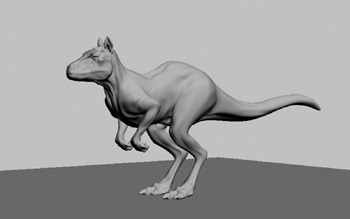
\includegraphics[width=0.8\linewidth]{./assets/AO_DiffuseOnly.jpg}
  \label{fig:AO1_diffuse}
\end{subfigure}%
\begin{subfigure}{.5\columnwidth}
  \centering
  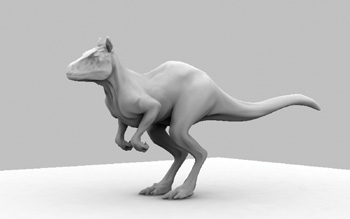
\includegraphics[width=0.8\linewidth]{./assets/AO_FullAO.jpg}
  \label{fig:AO1_fullao}
\end{subfigure}
\caption{[LEFT] Diffuse Shading, [RIGHT] Ambient Occlusion and Diffuse Shading }
\label{fig:AO1}
\end{figure}

\begin{comment}
%%%%%%%%%%%%%%%%%%%%%%%%%%%%%%%%%%%%%%%%%%%%%%%%%%%%%%%%%%%%%%%%%%%%%%%%%%%%%%%%%%%%%%%%%%%%%%%%%%%%%%%%%%%%
%%%%%%%%%%%%%%%%%%%%%%%%%%%%%%%%%%%%%%%%%%%%%%%%%%%%%%%%%%%%%%%%%%%%%%%%%%%%%%%%%%%%%%%%%%%%%%%%%%%%%%%%%%%%
\section{VGG08 Batch Norm Classifier Architecture}
%%%%%%%%%%%%%%%%%%%%%%%%%%%%%%%%%%%%%%%%%%%%%%%%%%%%%%%%%%%%%%%%%%%%%%%%%%%%%%%%%%%%%%%%%%%%%%%%%%%%%%%%%%%%
%%%%%%%%%%%%%%%%%%%%%%%%%%%%%%%%%%%%%%%%%%%%%%%%%%%%%%%%%%%%%%%%%%%%%%%%%%%%%%%%%%%%%%%%%%%%%%%%%%%%%%%%%%%%

The classifier model architecture is a VGG08 model with batch normalization and 100 output features. This model can be thought of two connected parts, a feature learner and classifier.  The feature learner is the 5 layers of convolutions and the classifier is the 3 fully connected linear layers.\\  
In more detail the architecture is for the feature learner: 
\begin{enumerate}
\item 64 x Conv2D(3x3) - BatchNorm - ReLU - Max Pool
\item 128 x Conv2D(3x3) - BatchNorm - ReLU - Max Pool
\item 256 x Conv2D(3x3) - BatchNorm - ReLU - Max Pool
\item 512 x Conv2D(3x3) - BatchNorm - ReLU - Max Pool
\item 512 x Conv2D(3x3) - BatchNorm - ReLU - Max Pool
\end{enumerate}
The features (512x3x3) are then fed into a classifier of architecture: 
\begin{itemize}
\item Linear (in: 512x3x3, out: 100) - ReLU - Dropout
\item Linear(100,100) - BatchNorm - Dropout
\item Linear(100, 5)
\item LogSoftmax
\end{itemize}

%%%%%%%%%%%%%%%%%%%%%%%%%%%%%%%%%%%%%%%%%%%%%%%%%%%%%%%%%%%%%%%%%%%%%%%%%%%%%%%%%%%%%%%%%%%%%%%%%%%%%%%%%%%%
\subsection{Loss functions used}
%%%%%%%%%%%%%%%%%%%%%%%%%%%%%%%%%%%%%%%%%%%%%%%%%%%%%%%%%%%%%%%%%%%%%%%%%%%%%%%%%%%%%%%%%%%%%%%%%%%%%%%%%%%%
\subsection{All data rendering and generation methods}
%%%%%%%%%%%%%%%%%%%%%%%%%%%%%%%%%%%%%%%%%%%%%%%%%%%%%%%%%%%%%%%%%%%%%%%%%%%%%%%%%%%%%%%%%%%%%%%%%%%%%%%%%%%%
\end{comment}
\begin{comment}
%%%%%%%%%%%%%%%%%%%%%%%%%%%%%%%%%%%%%%%%%%%%%%%%%%%%%%%%%%%%%%%%%%%%%%%%%%%%%%%%%%%%%%%%%%%%%%%%%%%%%%%%%%%%
%%%%%%%%%%%%%%%%%%%%%%%%%%%%%%%%%%%%%%%%%%%%%%%%%%%%%%%%%%%%%%%%%%%%%%%%%%%%%%%%%%%%%%%%%%%%%%%%%%%%%%%%%%%%
\subsubsection{OpenGL}
%%%%%%%%%%%%%%%%%%%%%%%%%%%%%%%%%%%%%%%%%%%%%%%%%%%%%%%%%%%%%%%%%%%%%%%%%%%%%%%%%%%%%%%%%%%%%%%%%%%%%%%%%%%%
We created an OpenGL \cite{Shreiner:2013:OPG:2544032} based renderer in C++ and bound it to pyTorch and python using FFI.  OpenGL is a 3D API that is cross platform and allows for direct programming of GPUs.  
\end{comment}
%%%%%%%%%%%%%%%%%%%%%%%%%%%%%%%%%%%%%%%%%%%%%%%%%%%%%%%%%%%%%%%%%%%%%%%%%%%%%%%%%%%%%%%%%%%%%%%%%%%%%%%%%%%%

%%%%%%%%%%%%%%%%%%%%%%%%%%%%%%%%%%%%%%%%%%%%%%%%%%%%%%%%%%%%%%%%%%%%%%%%%%%%%%%%%%%%%%%%%%%%%%%%%%%%%%%%%%%%
\subsubsection{Global Illumination and Mitsuba}\label{mitsuba_section}
%%%%%%%%%%%%%%%%%%%%%%%%%%%%%%%%%%%%%%%%%%%%%%%%%%%%%%%%%%%%%%%%%%%%%%%%%%%%%%%%%%%%%%%%%%%%%%%%%%%%%%%%%%%%
Global illumination (GI) refers to rendering methods that try to take into account inter-surface reflection. It is different from faster approximate methods that only simulate direct lighting.  GI derives its accuracy from its ability to take into account the light that arrives at a surface not just directly from a light source, but from light that has been reflected off of other surfaces as well. Different surface materials have different reflection characteristics that effect how much sampling must be done in order to converge to the right solution.  We are fortunate in that in our dataset all of our surfaces are diffuse and there are few surfaces capable of reflecting light onto the objects in the scene.  This means the sample counts needed to converge our scenes represent the low end needed to adequately simulate an image in a GI renderer. Typically, thousands of samples are necessary to get a noise free image\footnote{Usually for scenes with highly reflective surfaces and small bright light sources}.\\

In order to simulate global illumination in our experiments, we used an open source global illumination renderer called Mitsuba\cite{Mitsuba}.  It generates high quality images that it creates by trying to solve the rendering equation \cite{Kajiya:1984:RTV:800031.808594} by bouncing many light rays throughout the 3D scene.  The more samples it takes, the closer to the solution and the more realistic the image becomes.  This all comes at a high computation cost with the images take many times longer to compute than with rasterization methods such as OpenGL.  

%%%%%%%%%%%%%%%%%%%%%%%%%%%%%%%%%%%%%%%%%%%%%%%%%%%%%%%%%%%%%%%%%%%%%%%%%%%%%%%%%%%%%%%%%%%%%%%%%%%%%%%%%%%%
%%%%%%%%%%%%%%%%%%%%%%%%%%%%%%%%%%%%%%%%%%%%%%%%%%%%%%%%%%%%%%%%%%%%%%%%%%%%%%%%%%%%%%%%%%%%%%%%%%%%%%%%%%%%
\section{Training Data creation}
%%%%%%%%%%%%%%%%%%%%%%%%%%%%%%%%%%%%%%%%%%%%%%%%%%%%%%%%%%%%%%%%%%%%%%%%%%%%%%%%%%%%%%%%%%%%%%%%%%%%%%%%%%%%
%%%%%%%%%%%%%%%%%%%%%%%%%%%%%%%%%%%%%%%%%%%%%%%%%%%%%%%%%%%%%%%%%%%%%%%%%%%%%%%%%%%%%%%%%%%%%%%%%%%%%%%%%%%%
Direct comparisons between rendering techniques and real images could not be done without creating a dataset that allows for it.  We were able to identify the NYU Object Recognition Benchmark (NORB) dataset \cite{LeCun:2004:LMG:1896300.1896315} as a good starting point. Despite its age, it has enough advantages for it to be useful.  It is also simple and small enough to allow for recreation of each photograph shot for shot.  A characteristic that makes NORB even more attractive is that the object location, rotation and camera placement are known for every image.

However, the NORB dataset is black and white, and we wanted to also collect data on a colorized set of images. In order to do this, we generated 
%%%%%%%%%%%%%%%%%%%%%%%%%%%%%%%%%%%%%%%%%%%%%%%%%%%%%%%%%%%%%%%%%%%%%%%%%%%%%%%%%%%%%%%%%%%%%%%%%%%%%%%%%%%%
\subsubsection{NORB Dataset}
%%%%%%%%%%%%%%%%%%%%%%%%%%%%%%%%%%%%%%%%%%%%%%%%%%%%%%%%%%%%%%%%%%%%%%%%%%%%%%%%%%%%%%%%%%%%%%%%%%%%%%%%%%%%
\begin{comment}
Training with real data then using the model to classify real test images gives the baseline performance.  Training the vgg08 batchnorm model with NORB photographs from one lighting condition results in 4050 training images. Training with this data results in an accuracy of 96.86\% on test images from the same lighting condition.
\end{comment}

\begin{figure}[h!]
\centering
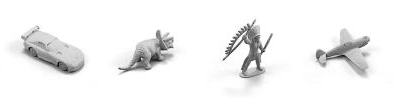
\includegraphics[width=1.0\columnwidth]{./assets/NORBTestSmall.png}
\caption{A sample of the NORB test dataset. Note the dark shadows under some of the models, animals in particular.}
\label{fig:norb-samples}
\end{figure}
%The NORB \cite{LeCun:2004:LMG:1896300.1896315} dataset is quite old and simple and is not used to train and test classifiers anymore.  However the nature of the dataset allows it to be very useful in experimenting with rendering techniques due to the characteristics of the data.\\

The objects within the NORB dataset are a set of 50 toys split into a 25 object training set and a 25 object test set. The dataset is stereo photographs of the objects on a turntable in 6 controlled lighting conditions, 18 uniform rotations and 9 elevations. This results in a dataset with 48,600 stereo pictures.  We focus on just the 25 objects in the training set consisting of $6\cdot9\cdot18\cdot25=24,300$ images in the dataset we generated for our tests.  We also confined our dataset to one lighting condition to keep it uniform across all images.  This reduces the image count in the training dataset to 4,050 images.   The toys were painted a uniform color with a matte paint. This was intended to prevent texture from being used in classification. \\

All of the properties listed above facilitate a recreation of the original scenes through 3D rendering. We know the pose, location and surface of the objects as well as the location of the camera. We set the material properties of the objects to be a uniform color and diffusely reflective. This leaves us with the task of accurately recreating the geometry of the toys in 3D.

After acquiring and scanning the objects\footnote{We acquired some of the toys by asking the original authors for them with the missing ones located on EBay. Examples of the toys are shown in figure \ref{fig:norbscans}.  We used a high resolution 3D scanner to scan in the objects.  The scanner is shown in Figure \ref{fig:david}.  The models were then cleaned up and uniformly scaled to fit into a unit cube with the bottom center at the origin.  Models setup this way allow for a standard way to rotate the objects and place them so they touch the ground plane.}, we created a matching g-buffer for every image in the training dataset.  

Mitsuba produced the G-Buffers and shaded images at a resolution of 768x768 for each image.  The images and buffers were then cropped and resized such that the bounding box of the mesh pixels fit into an 80x80 pixel square, with the final image itself being a 96x96 pixel square. This mirrors the procedure done for the real NORB dataset.  \footnote{Early tests did not have this final processing step, and resulted in lower accuracy test results due to the difference between the formatting of the synthetic training data and the real test data.}

This results in a one-to-one mapping between each image in the synthetic training dataset and image in the real training dataset.  This allows different experiments using the g-buffers to assume that the 3D scenes are identical, ensuring the differences in synthesized output can be directly attributed to shading technique. 
It also allows for direct comparison between rendered images and the real images because the images are not just of the same object but are an accurate recreation of each photograph in the original dataset.

The NORB dataset does have its shortcomings. The dataset is black and white, low resolution, and it small in size. While these are drawbacks, it does not prevent us from conducting experiments on rendering methods and comparing them to each other.  The dataset is simple and allows for more controllable experiments.  However, it does make it harder to conclude that a method that works for this dataset will also work for datasets with more complex imagery.



\begin{figure}[h!]
\centering
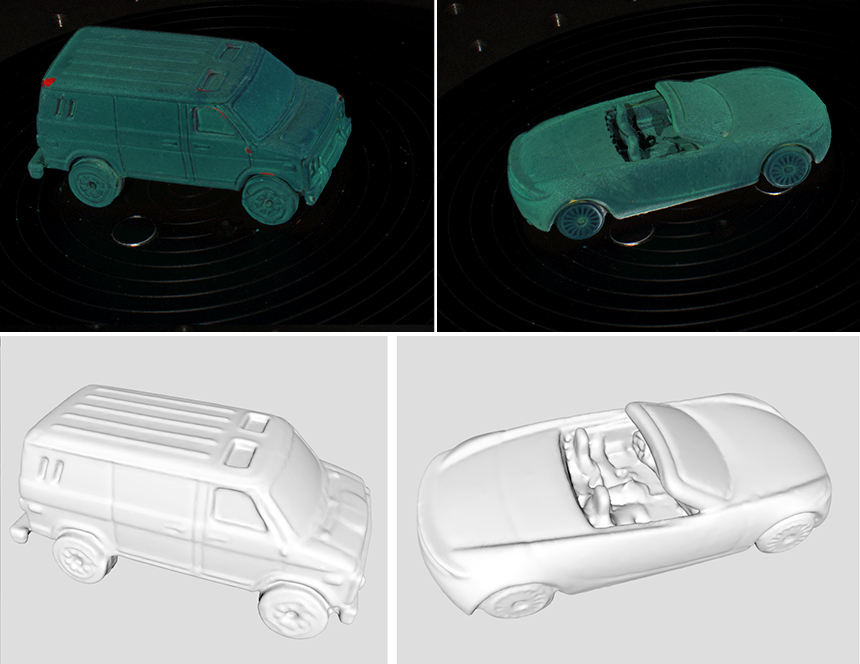
\includegraphics[width=0.8\linewidth]{./assets/ToysScannerAndScan.png}
\caption{Top: Two pictures of NORB Toys on the turntable taken from one of scanner's cameras.\\ Bottom: Results of scan when cleaned and reduced to 65,000 vertices.}
\label{fig:norbscans}
\end{figure}

\begin{figure}[h!]
\centering
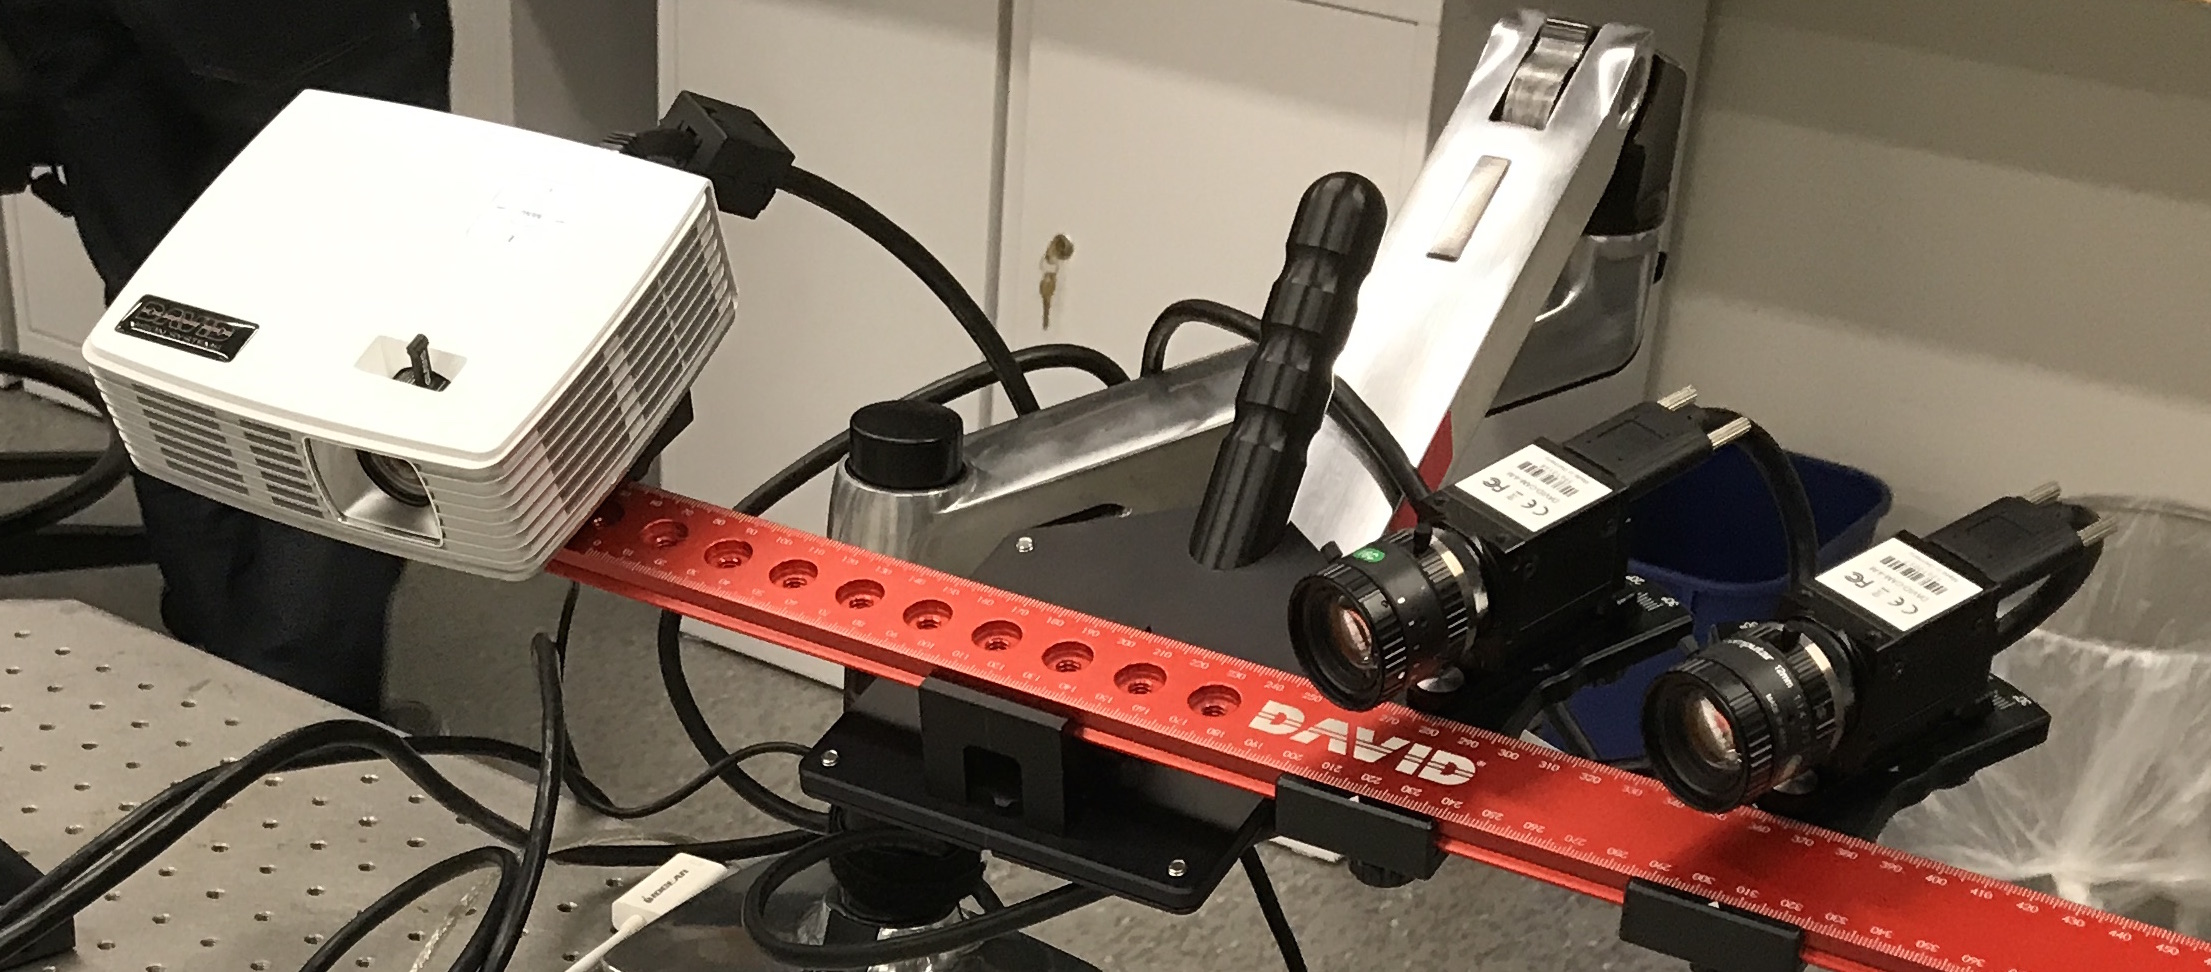
\includegraphics[width=0.8\columnwidth]{./assets/david_scanner.JPG}
\caption{A picture of the scanner setup used to generate 3D models of the physical toys. The turntable used to rotate the toys to get a full 360-degree view is not shown here.}
\label{fig:david}
\end{figure}

%%%%%%%%%%%%%%%%%%%%%%%%%%%%%%%%%%%%%%%%%%%%%%%%%%%%%%%%%%%%%%%%%%%%%%%%%%%%%%%%%%%%%%%%%%%%%%%%%%%%%%%%%%%%
%%%%%%%%%%%%%%%%%%%%%%%%%%%%%%%%%%%%%%%%%%%%%%%%%%%%%%%%%%%%%%%%%%%%%%%%%%%%%%%%%%%%%%%%%%%%%%%%%%%%%%%%%%%%
\section{Experiments}
%%%%%%%%%%%%%%%%%%%%%%%%%%%%%%%%%%%%%%%%%%%%%%%%%%%%%%%%%%%%%%%%%%%%%%%%%%%%%%%%%%%%%%%%%%%%%%%%%%%%%%%%%%%%
%%%%%%%%%%%%%%%%%%%%%%%%%%%%%%%%%%%%%%%%%%%%%%%%%%%%%%%%%%%%%%%%%%%%%%%%%%%%%%%%%%%%%%%%%%%%%%%%%%%%%%%%%%%%
In our experiments, we use increasingly complex simulation methods for rendering our images.  We start with just a silhouette as training data and we then incrementally increase the sophistication level of the simulation during rendering.  We then add complexity such as shading, shadowing and global illumination. Finally, we use a form of a denoising autoencoder to learn cleanup  and refine GI based images.\\ 

In order to properly measure the impact of these various techniques, it is important to use a single classifier architecture across all experiments.

\begin{figure}[h!]
\centering
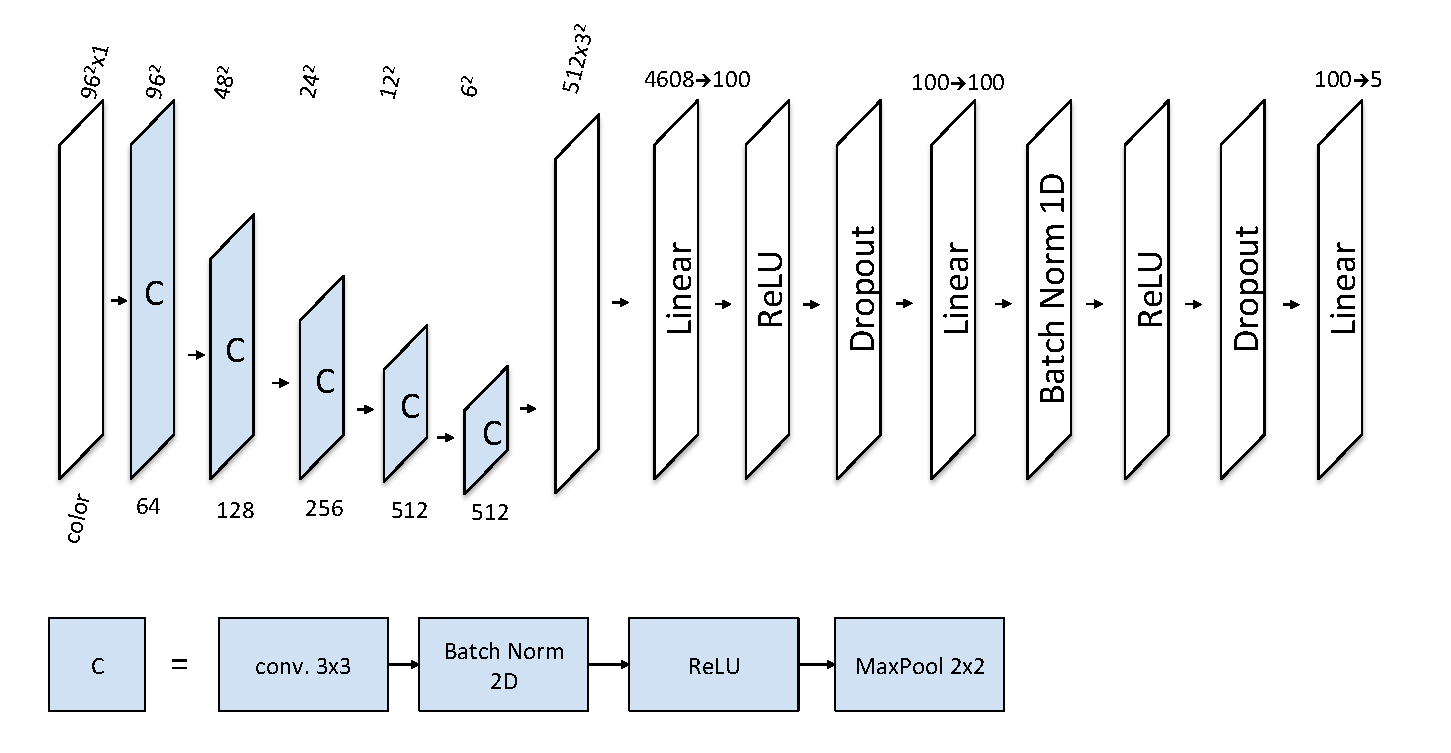
\includegraphics[width=1.0\columnwidth]{./assets/vgg08_diagram.pdf}
\caption{Architecture of VGG08 Batch Norm Classifier}
\label{fig:VGG_DAIGRAM}
\end{figure}
The network architecture we use is a simplification of the VGG network\cite{DBLP:journals/corr/SimonyanZ14a}.  We reduce it to having 8 learnable layers which include 5 convolutional layers in the feature learner and three classification linear layers.   
The 5 scores given by the last learnable layer are then put through a Log Softmax and a Negative Log Likelyhood loss. %% TODO: Might be worth writing out the equation for these -- your call 
Figure \ref{fig:VGG_DAIGRAM} has more detail.\\

%%%%%%%%%%%%%%%%%%%%%%%%%%%%%%%%%%%%%%%%%%%%%%%%%%%%%%%%%%%%%%%%%%%%%%%%%%%%%%%%%%%%%%%%%%%%%%%%%%%%%%%%%%%%
\subsubsection{Training on Real Images}
%%%%%%%%%%%%%%%%%%%%%%%%%%%%%%%%%%%%%%%%%%%%%%%%%%%%%%%%%%%%%%%%%%%%%%%%%%%%%%%%%%%%%%%%%%%%%%%%%%%%%%%%%%%%
To establish a target performance level that we can measure our shading methods against, we train our classifier on the NORB dataset. However, we filter out all but one lighting condition for both test and training data.  This reduces the test and training datasets to 4,050 images each.  The synthetic g-buffer set is the same size.  
 The goal is to see if any of the classifiers training on synthetic data can achieve similar performance to that of a classifier trained on real data.  See figure \ref{fig:norb-samples} for examples of the NORB images.\\

Training with the reduced photographic dataset yields a 95.01\% accuracy.  This score is achieved by training for 200 epochs without any data augmentation and a learning rate of 5e-5. The only data modifications are image normalization for renderer outputs and converting the g-buffer depth maps to be in the linear range of $[0,1]$.  For the rest of the experiments when we train this classifier, the epoch count remains the same and the training data is not augmented.\\  

By keeping the training the same across experiments, we isolate any difference in scores to be only attributable to shading.
%%%%%%%%%%%%%%%%%%%%%%%%%%%%%%%%%%%%%%%%%%%%%%%%%%%%%%%%%%%%%%%%%%%%%%%%%%%%%%%%%%%%%%%%%%%%%%%%%%%%%%%%%%%%
\subsection{Different Rendering Methods}
%%%%%%%%%%%%%%%%%%%%%%%%%%%%%%%%%%%%%%%%%%%%%%%%%%%%%%%%%%%%%%%%%%%%%%%%%%%%%%%%%%%%%%%%%%%%%%%%%%%%%%%%%%%%
\begin{table}[]
\centering
\label{tblnonGI}
\begin{tabular}{|l|r|r|}
\hline
\multicolumn{1}{|c|}{\textbf{Input}} & \multicolumn{1}{r|}{\textbf{Accuracy}} & \multicolumn{1}{r|}{\textbf{$\Delta$ vs Real}} \\ \hline
Albedo Only                          & 46.20\%                                & 48.81 / 48.63\%                                \\
Learned SH Shading                   & 48.52\%                                & 46.49 / 51.07\%                                \\
SH Shading + AO                      & 55.80\%                                & 39.21 / 58.73\%                                \\
2 Bounce (Direct Lighting)           & 55.78\%                                & 39.23 / 58.71\%                                \\
\textbf{Real Images}                          & \textbf{95.01}\%                                & \textbf{0 / 100.00}\%                                   \\ \hline
\multicolumn{3}{|c|}{\textbf{Performance Of Basic Rendering Methods}}                                                          \\ \hline
\end{tabular}
\caption{Performance of rendering methods that currently possible to do in real-time. Albedo Only is passing in the albedo map (see figure \ref{fig:GBUFFER_ALBEDO}). Learned SH Shading is unshadowed shading. SH Shading + AO is unshadowed shading with AO composited with the result. See section \ref{sec:learned_sh} for more detail. 2 Bounce (Direct Lighting) is a shading plus shadowing that is described in section \ref{sec:2bounce}. $\Delta$ vs Real has two numbers: the left is the difference in accuracy from the best result of each method compared to using real data, and the right is the percentage of the real data trained classifier's accuracy that the method achieves.  100\% would mean that the method would have achieved 95.01\% accuracy when training a classifier.  } 
\end{table}



%%%%%%%%%%%%%%%%%%%%%%%%%%%%%%%%%%%%%%%%%%%%%%%%%%%%%%%%%%%%%%%%%%%%%%%%%%%%%%%%%%%%%%%%%%%%%%%%%%%%%%%%%%%%
\subsubsection{No Shading - Albedo Only}
%%%%%%%%%%%%%%%%%%%%%%%%%%%%%%%%%%%%%%%%%%%%%%%%%%%%%%%%%%%%%%%%%%%%%%%%%%%%%%%%%%%%%%%%%%%%%%%%%%%%%%%%%%%%
To establish a baseline for minimal performance, we train with just the albedo map as input.  This is equivalent to an unshaded scene and can establish what the classifier can learn without any shading information. See figure \ref{fig:GBUFFER_ALBEDO}.  The score achieved is 46.20\%. All of the other methods score better than this, which confirms that simulating how light interacts with the object is significant.
%%%%%%%%%%%%%%%%%%%%%%%%%%%%%%%%%%%%%%%%%%%%%%%%%%%%%%%%%%%%%%%%%%%%%%%%%%%%%%%%%%%%%%%%%%%%%%%%%%%%%%%%%%%%
\subsubsection{Shading Extracted from Rendering Through Learnable Spherical Harmonics}\label{sec:learned_sh}
%%%%%%%%%%%%%%%%%%%%%%%%%%%%%%%%%%%%%%%%%%%%%%%%%%%%%%%%%%%%%%%%%%%%%%%%%%%%%%%%%%%%%%%%%%%%%%%%%%%%%%%%%%%%
\begin{figure}[h!]
\centering
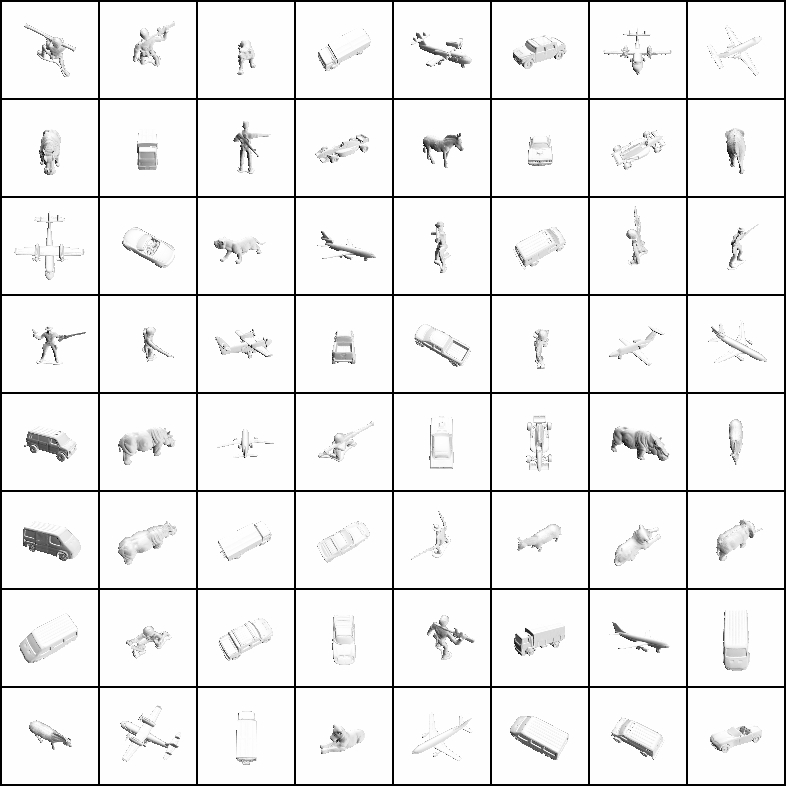
\includegraphics[trim={0 0 392px 687px},clip,width=1.0\columnwidth]{./assets/SH_LitTrainingData.jpg}
\caption{Learned spherical harmonics lighting and diffuse shading without albedo.  Notice that it cannot learn the albedo of the object and it affects what lighting function it learns.  The ground plane normal dominates the loss and biases the lighting distribution.}
\label{fig:SH_ONLY}
\end{figure}

\begin{figure}[h!]
\centering
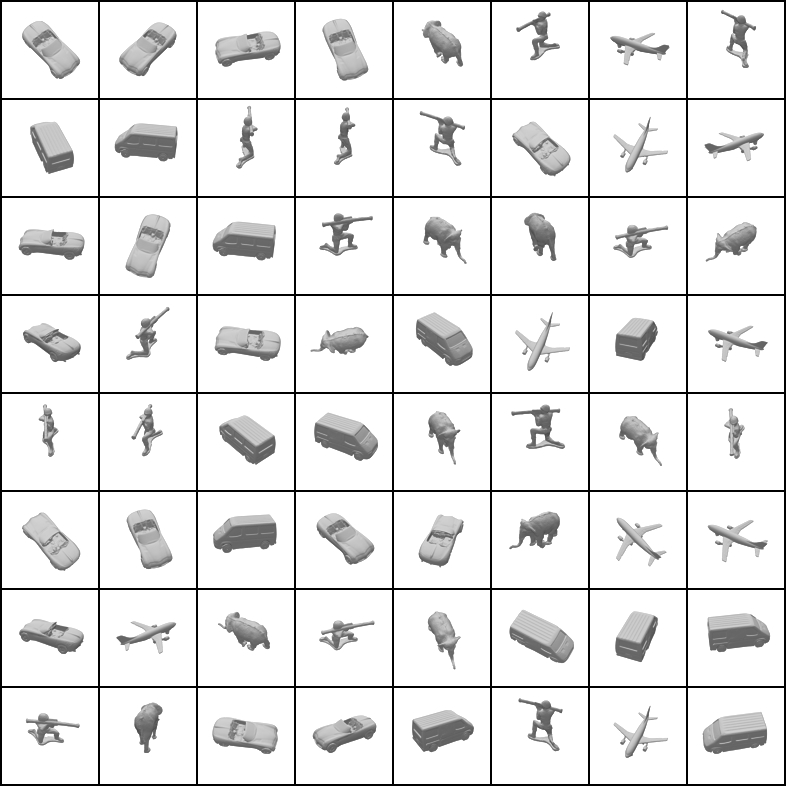
\includegraphics[trim={0 0 392px 687px},clip,width=1.0\columnwidth]{./assets/Best_Learned_SH_Image_Training_Data.jpg}
\caption{Albedo multiplied by learned spherical harmonics lighting with diffuse shading.}
\label{fig:SH_and_Albedo}
\end{figure}


\begin{figure}[h!]
\centering
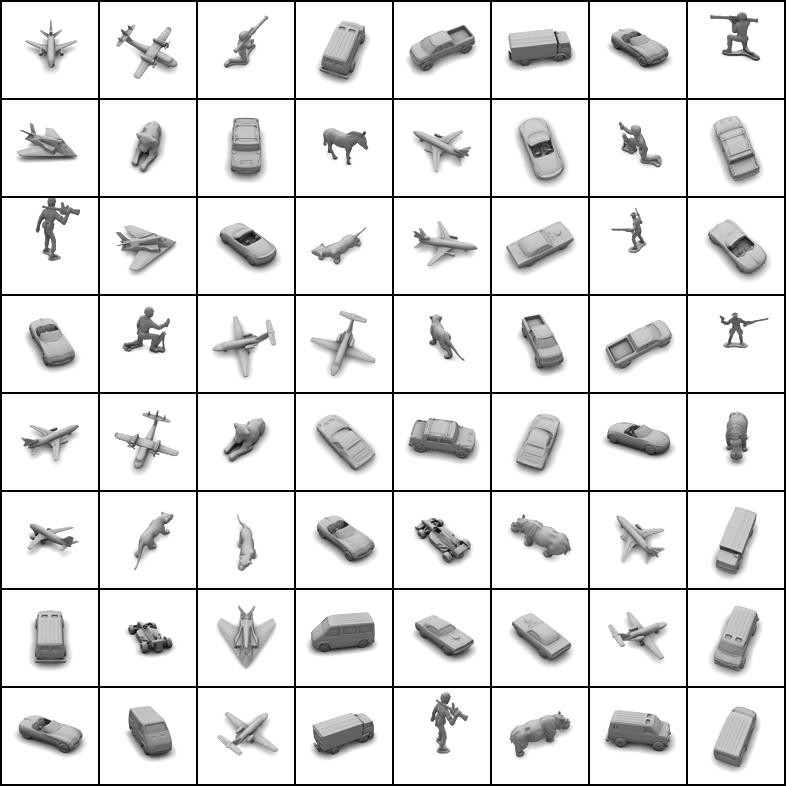
\includegraphics[trim={0 0 392px 687px},clip,width=1.0\columnwidth]{./assets/Learned_SH_plus_AO_and_Albedo.jpg}
\caption{Learned spherical harmonics lighting with albedo and ambient occlusion and diffuse shading.}
\label{fig:SH_AO_ALBEDO}
\end{figure}
The next step beyond albedo-only rendering is shading without shadows. We could not get Mitsuba to output shading without shadows, so we chose to learn the shading given a full rendering.  We did this with a Spherical Harmonics (SH) module that enabled learning the 9 parameters to the 3 bands of functions.  These are enough bases to learn diffuse surfaces within a 99\% accuracy \cite{Shreiner:2013:OPG:2544032}.\\

The input data is a normal buffer and an albedo buffer.  The target is the full 128 sample GI render of the scene.  The SH module takes the normals as input and outputs an intensity.  That is then multiplied by the albedo and passed into a L1 loss function.  The loss is then backpropogated through the SH layer to adjust the shading.\\

The result is a network that has learned the shading of the objects based upon the lighting in the target images.  The output also has the desired property of not having any shadows and allows us to test for shading based on surface normals.\\

For examples of a learned SH lighting combined with albedo, see figure \ref{fig:SH_and_Albedo}.  See figures \ref{fig:SH_ONLY}, \ref{fig:SH_and_Albedo} and \ref{fig:SH_AO_ALBEDO} to see the effects of combining different channels. Training with just the composition of SH and albedo results in an accuracy of 48.52\%.   Compositing the SH shaded surface with the albedo and AO maps gives the most realistic result.  The classifier trained with the composition of all three has an accuracy of 55.80\%, which is indeed higher than just compositing SH and albedo.  This shows that at least some form of shadows are important for classification.


%%%%%%%%%%%%%%%%%%%%%%%%%%%%%%%%%%%%%%%%%%%%%%%%%%%%%%%%%%%%%%%%%%%%%%%%%%%%%%%%%%%%%%%%%%%%%%%%%%%%%%%%%%%%
\subsubsection{Two Bounce Mitsuba}\label{sec:2bounce}
%%%%%%%%%%%%%%%%%%%%%%%%%%%%%%%%%%%%%%%%%%%%%%%%%%%%%%%%%%%%%%%%%%%%%%%%%%%%%%%%%%%%%%%%%%%%%%%%%%%%%%%%%%%%

\begin{figure}[h!]
\centering
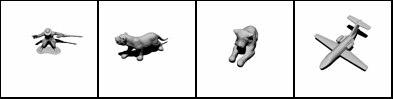
\includegraphics[width=1.0\columnwidth]{./assets/2bounce_small.png}
\caption{Two Bounce Rendering.  Notice it is the equivalent to a shadow mapped scene and differs from the AO composited scenes by the sharpness of the shadows. This is due to the scene using a single directional light.}
\label{fig:2BOUNCE}
\end{figure}
% TODO: this paragraph bounces between past and present tense, reads kind of weird
Now that we have seen that an approximate shadow (Ambient Occlusion) helps the classifier, we add shadows to the synthetic dataset. However, we don't want inter-reflections and global illumination, as we test that separately.  This can be achieved in Mitsuba by limiting how many bounces the rays take during simulation.  We only allow the rays fired through the screen to hit an object, bounce, and see if it hits a light source.  There are no secondary bounces to allow indirect lighting to illuminate the object. We also choose to use a single directional light to create very hard shadows.  This will allow us to contrast the performance of hard shadows and soft shadows which are both present in the real dataset.  This is also a good approximation of what a video game engine might produce and can be used as a proxy for video game engine generated synthetic data.  See figure \ref{fig:2BOUNCE} for examples of this rendering method.  The resulting performance from training with this data was very similar to SH composited with albedo and AO.  It yields an accuracy of 55.78\%.  An possible explanation could be that the real data has one sharp shadow from an overhead light and a soft shadow from another. Additionally, ambient occlusion is a good approximation of the dominant light source in the scene which is large with uniform brightness and occupies a large part of the hemisphere surrounding the object.


%%%%%%%%%%%%%%%%%%%%%%%%%%%%%%%%%%%%%%%%%%%%%%%%%%%%%%%%%%%%%%%%%%%%%%%%%%%%%%%%%%%%%%%%%%%%%%%%%%%%%%%%%%%%
\subsubsection{Varying Sample Count in the Mitsuba Path Tracer}
%%%%%%%%%%%%%%%%%%%%%%%%%%%%%%%%%%%%%%%%%%%%%%%%%%%%%%%%%%%%%%%%%%%%%%%%%%%%%%%%%%%%%%%%%%%%%%%%%%%%%%%%%%%%
\begin{table*}[]
\centering

\begin{tabular}{|l|r|r|r|r|}
\hline
\multicolumn{1}{|c|}{\textbf{Input}} & \multicolumn{1}{c|}{\textbf{1 Sample}} & \multicolumn{1}{c|}{\textbf{4 Sample}} & \multicolumn{1}{c|}{\textbf{128 Sample}} & \multicolumn{1}{c|}{\textbf{$\Delta$ vs Real}} \\ \hline
Mitsuba& 57.21\%                                & 72.89\%                                 & 74.84\%                                   & 20.18/78.77\%                               \\
Denoised& 71.48\%                                & 73.56\%                                 & N/A                                       & 21.45/77.42\%                                \\
Single GAN& 72.84\%                                & 77.65\%                                 & 75.26\%                                   & \textbf{17.36/81.73\%}                            \\
Multiple GAN& 85.23\%                                   & 84.37\%                                 & 87.33\%                                   & \textbf{7.68/91.92\%}                            \\ \hline
\multicolumn{5}{|c|}{\textbf{Performance of GI Rendered Refined Images}}                                                                                                                                             \\ \hline
\end{tabular}
\caption{Comparison of GI Rendered Refined Image Performance. The GAN output refers to if only one GAN was used to refine the dataset or if the dataset was expanded by multiple GANs. $\Delta$ vs Real has two numbers. The left is the difference in accuracy from the best result of each method compared to using real data (Real achieved \textbf{95.01\%}). See section \ref{sec:gans} for further details.  The second number is the percentage of the real data trained classifier's accuracy that the method achieves.  100\% would mean that the method would have achieved 95.01\% accuracy when training a classifier. See section \ref{sec:multigans} for more details. Bold values represent values that are better than the accuracy of the best quality GI rendering (128 Sample Mitsuba).}
\label{tblallrefined}
\end{table*}


\begin{figure}[h!]
\centering
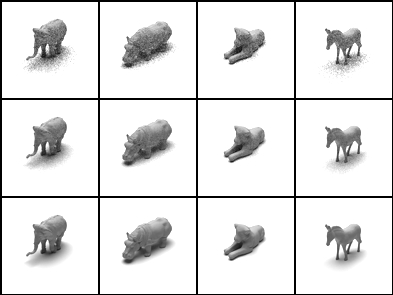
\includegraphics[width=1.0\columnwidth]{./assets/DifferentSampleCounts.png}
\caption{
Mitsuba renders at different sample counts. Top: 1 sample per pixel.  Middle: 4 samples per pixel.  Bottom: 128 samples per pixel
}
\label{fig:differentsamplesraw}
\end{figure}
\begin{comment}
\begin{figure}[h!]
\centering
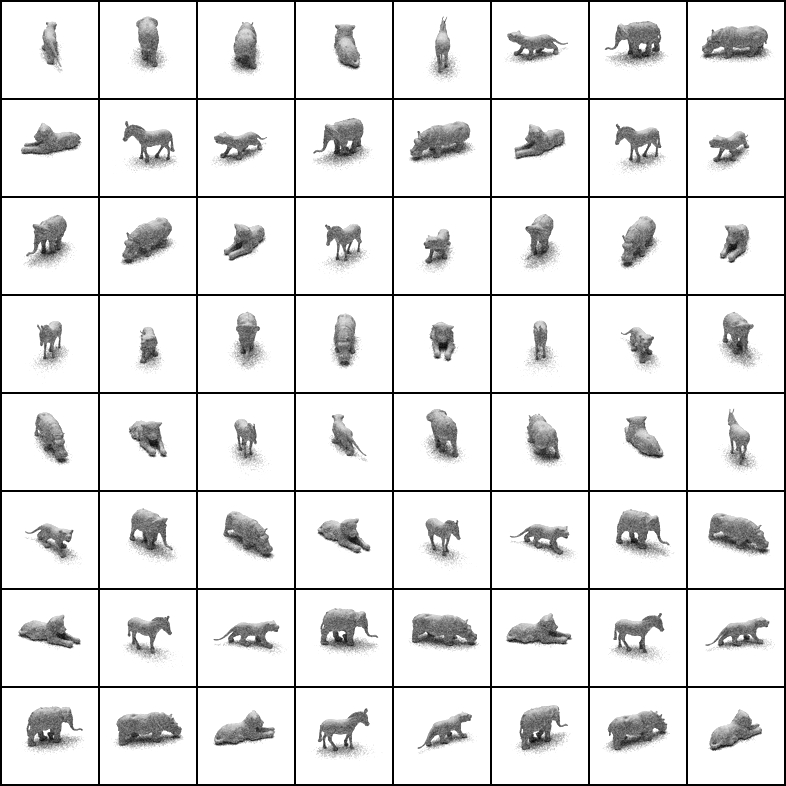
\includegraphics[trim={0 0 392px 687px},clip,width=1.0\textwidth]{./assets/traindata_1_sample.jpg}
\caption{Sample crop 1.}
\label{fig:crop1}
\end{figure}
\begin{figure}[h!]
\centering
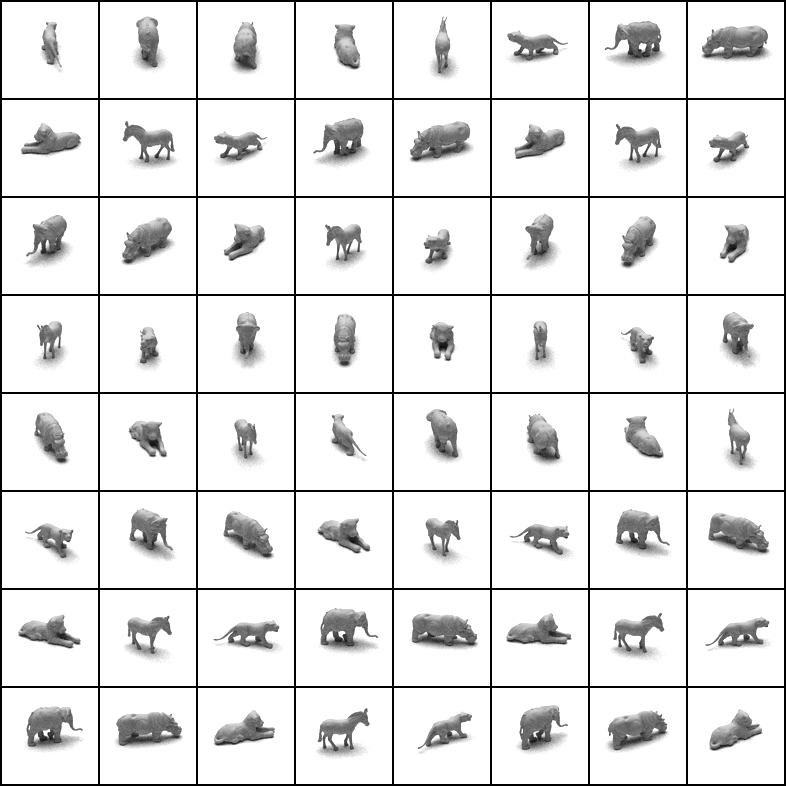
\includegraphics[trim={0 0 392px 687px},clip,width=1.0\textwidth]{./assets/traindata_4_sample.jpg}
\caption{Sample crop 4.}
\label{fig:crop4}
\end{figure}
\begin{figure}[h!]
\centering
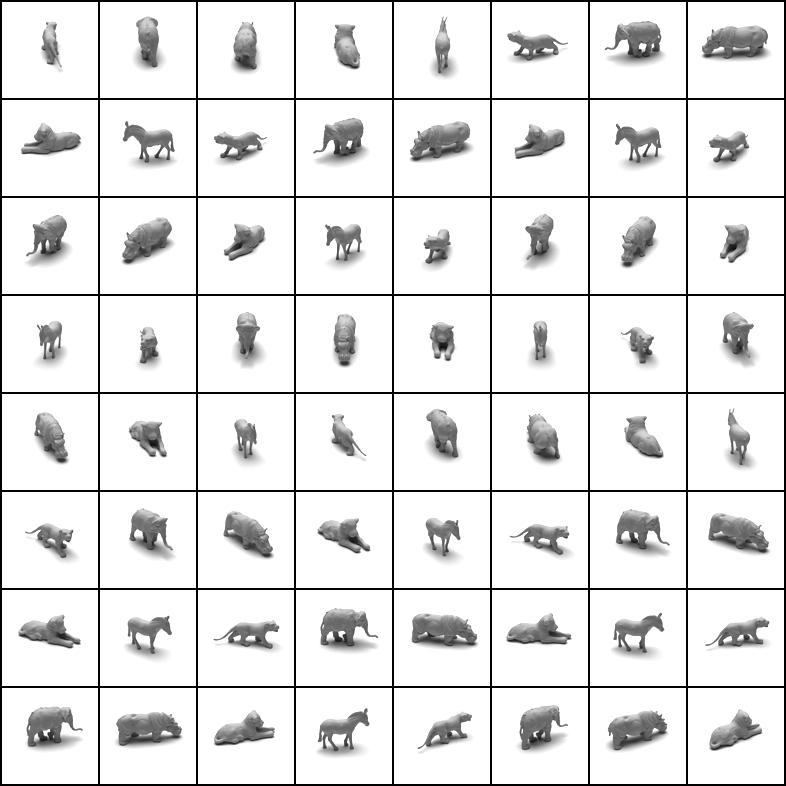
\includegraphics[trim={0 0 392px 687px},clip,width=1.0\textwidth]{./assets/traindata_target_128_sample.jpg}
\caption{Sample crop 128.}
\label{fig:crop128}
\end{figure}
\end{comment}


The last rendering feature that we add to achieve the most realism is allowing light to bounce inside the environment, reflecting off of surfaces and onto other objects in the scene.  Multiple bounces soften the shadows and allow light to come from below the object by reflecting off the ground plane.\\


A global illumination (GI) renderer creates images by firing rays through each pixel and checks for intersections with surfaces in the scene.  If it hits anything, it then fires many more rays emanating from the hit point and determines, inside a certain number of bounces, if the ray eventually hits a source of light.  It is important to realize that it takes many samples per bounce to accurately determine all of the incoming light arriving at a point upon an object's surface.
%Random sampling plays a heavy part in allowing the calculations to be efficient. 
However, if not enough samples are used it GI introduces noise into the final output. This is especially true for scenes composed of shiny surfaces and small bright light sources which induce light intensities along surfaces that can change very quickly.\\

We are fortunate that our scenes only involve surfaces that are diffuse and light sources that are relatively large compared to the illuminated objects.  Therefore it takes fewer samples to resolve the lighting for our images, as the intensity of reflected light varies slowly across diffuse surfaces.  However, we found we needed at least 128 samples per pixel to reduce the noise to be imperceptible. The high sample count is a significant problem with GI renderers, and is a major factor in the high computational cost per image.  For complex scenes with certain lighting and materials, it can take hours to generate an image.  Even in our simple scenes, it still took over a minute per image at 768x768 and 128 samples per pixel, while using one or four samples per pixel took only a few seconds a frame.\\

%Given that the full sample images are expensive to compute, can you use the noisy images? Is the noise in the image a problem for a convnet based classifier?  \footnote{This question was also asked by \cite{DBLP:journals/corr/VeeravasarapuRR16}. See Related work section}. To answer this question, 
We generated datasets using just one per pixel and four samples per pixel. We then used them to directly train a classifier.  We learned that the classifier can handle some noise without a performance penalty,  but too much noise hurts performance enough to negate the fact that a GI renderer is being used.  The baseline comparison is the 128 ``noiseless'' image, which achieves a performance of 74.84\%.  The 4-sample image is close in performance but also does not have much noise.  It gets an accuracy of 72.89\%, which is quite close to 128 samples while being 32 times less computation.  The single sample image only achieves an accuracy of 57.21\%, which is significantly worse and is in the same order of accuracy as much cheaper rendering methods.  However, the single sample per pixel image has a significant amount of noise.  The difference between the 1 and 4 sample images is most apparent at the edges. Four samples seems to be enough to have resolvable edges while only 1 sample was insufficient to define a border between shadow and unshadowed regions. See figure \ref{fig:differentsamplesraw} to see the difference in image quality based upon sample count. 
%Mitsuba is a free open source path tracer that allows for the control of how many bounces a light can take before it no longer is simulated and it allows for how many samples are taken per pixel.\\

%%%%%%%%%%%%%%%%%%%%%%%%%%%%%%%%%%%%%%%%%%%%%%%%%%%%%%%%%%%%%%%%%%%%%%%%%%%%%%%%%%%%%%%%%%%%%%%%%%%%%%%%%%%%
\subsubsection{Train on Denoised Images} \label{denoising}
%%%%%%%%%%%%%%%%%%%%%%%%%%%%%%%%%%%%%%%%%%%%%%%%%%%%%%%%%%%%%%%%%%%%%%%%%%%%%%%%%%%%%%%%%%%%%%%%%%%%%%%%%%%%
%Remembering that GI renderers are computationally expensive, we wanted to try techniques that would lower the render time. We wanted to see if we can get away with allowing the GI renderer to use fewer samples per pixel, and as a result, spend much less time computing images while maintaining the same performance from the dataset. 
Knowing that noisy images are still useful for training, we leverage the information in them to create a new image that performs better. Utilizing noisy images and equivalent ground truth versions, we ran experiments where we learned to denoise the images before training.  We implemented a simplified version of the network in \cite{Chaitanya:2017:IRM:3072959.3073601}.  We remove the recurrent part of the architecture because we are not learning animated sequences of images where noise removal has to be consistent across frames. The paper describes their architecture as a denoising auto-encoder with skip connections.  Our simplified version is shown in figure \ref{fig:denoise}. 
\begin{figure}[h!]
\centering
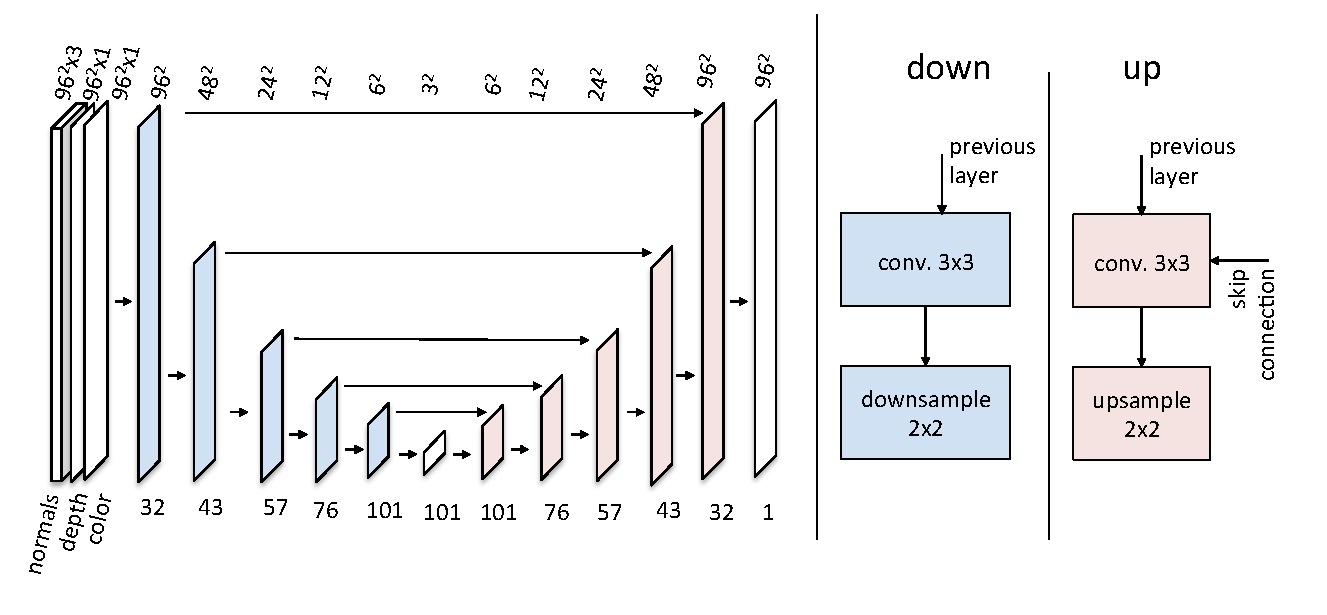
\includegraphics[width=1.0\columnwidth]{./assets/denoiser_diagram.pdf}
\caption{Architecture of Denoising Model}
\label{fig:denoise}
\end{figure}

The loss function used for denoising is Structured Similarity (SSIM)\cite{Wang04imagequality}. SSIM is typically used for image compression measurement, but also has been shown to be a good loss function for image comparison. The function for SSIM is given by
$$SSIM(p)=\frac{2\mu_x\mu_y + C_1}{\mu_x^2+\mu_y^2+C_1}\cdot\frac{2\sigma_{xy}+C_2}{\sigma_x^2+\sigma_y^2+C_2}$$
where $\mu$ is the mean of the pixel $p$ computed with a Gaussian filter, $\sigma^2$ is the variance and $\sigma_{xy}$ is the covariance. SSIM can be thought of as having a combination of three different measures: a luminance comparison for an approximate average difference in brightness,  a contrast comparison which measures a difference in brightness variance, and finally a structure comparison which uses a ration between the covariance and variance of the two images.  See \cite{DBLP:journals/corr/ZhangSYSLJF16} and \cite{DBLP:journals/corr/ZhaoGFK15} for details.\\

Denoising 1-sample images boosted accuracy from 57.21\% to 71.48\%, which is close to both 4 and 128 samples in performance while being much more accurate than other inexpensive rendering methods. Also, it is important to note that the rendering cost is two orders of magnitude lower than using the full sample count. 4 sample images, due to their low noise, only show a slight boost in performance.  The performance went from 72.89\% to 73.56\%.  The unadulterated 128 sample image achieved 74.84\%, which is only slightly better than the denoised low sample images.  Given that the denoising process takes milliseconds on a GPU \footnote{NVIDIA GeForce Titan X with 12GB or VRAM}, the cost of denoising is insignificant compared to taking more samples in a GI renderer.  See figure \ref{fig:differentsamplesraw} to see direct comparisons between images generated with different sample counts.\\

All of the results are listed in Table \ref{tblallrefined}.


\begin{comment}
\begin{table}[]
\centering
\label{tbldenoiseperf}
\begin{tabular}{|l|c|c|}
\hline
Samples        & 1             & 4             \\ \hline
Accuracy       & 71.48\%       & 73.56\%       \\ \hline
\multicolumn{3}{|c|}{Denoised Images Accuracy} \\ \hline
\end{tabular}
\caption{Performance of training on denoised images}
\end{table}
\end{comment}

%%%%%%%%%%%%%%%%%%%%%%%%%%%%%%%%%%%%%%%%%%%%%%%%%%%%%%%%%%%%%%%%%%%%%%%%%%%%%%%%%%%%%%%%%%%%%%%%%%%%%%%%%%%%
\subsection{Train on SimGAN images}
%%%%%%%%%%%%%%%%%%%%%%%%%%%%%%%%%%%%%%%%%%%%%%%%%%%%%%%%%%%%%%%%%%%%%%%%%%%%%%%%%%%%%%%%%%%%%%%%%%%%%%%%%%%%
\begin{comment}
\begin{figure}[h!]
\centering
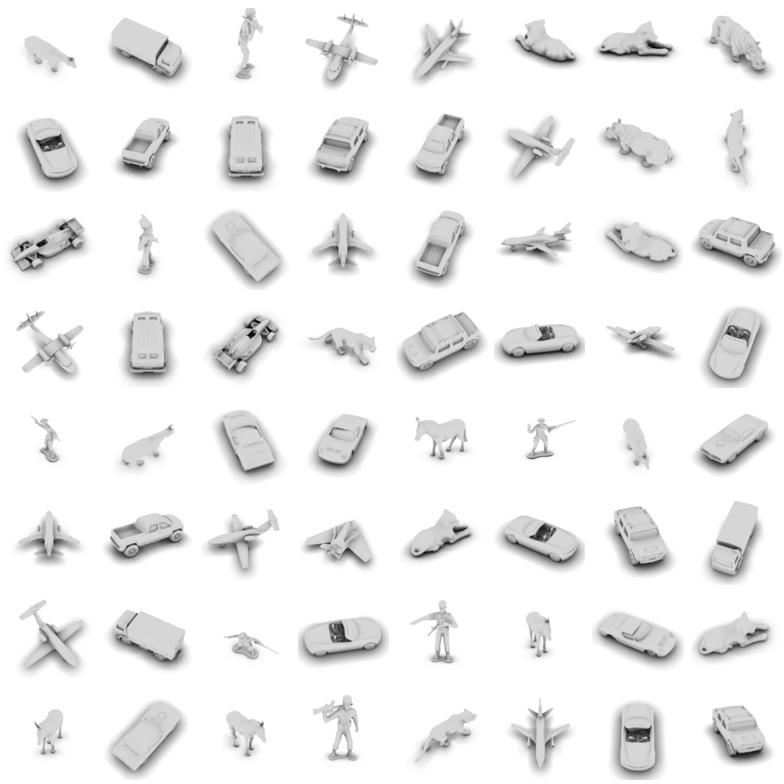
\includegraphics[trim={0 0 392px 687px},clip,width=1.0\textwidth]{./assets/mcm-train2.png}
\caption{Images generated with Mitsuba using an Ambient Occlusion rendering technique. This would have been part of the input and stored in the image input channel.}
\label{fig:AO_GAN_INPUT}
\end{figure}
\end{comment}

Another synthetic data generation technique that we explored involved the use of Generative Adversarial Networks \cite{2014arXiv1409.7495G}.  We chose to use a modified form of the architecture used in \cite{DBLP:journals/corr/ShrivastavaPTSW16}.   SimGAN is a novel GAN\cite{goodfellow} model, loss and training method used to refine input images.  The goal of the paper was to take existing datasets that are images created by a real-time renderer and to try and make them more like photographs. They achieve this by having their GAN learn a refiner that would alter the pixel inputs based upon the discriminator being able to correctly classify the refined image as real (photo) or fake (synthetic).  The SimGAN authors were trying to do more than classification, so they had a local loss function tailored to prevent the labels from being altered.  They made other changes to the traditional GAN training methods in order to stabilize the training and prevent the generator from outputting something useless.  For instance, they used a regularization loss which penalized refined images that looked too different from the original and they used a buffer of recent images to train from as further training stabilization.\\

We modified the SimGAN method for our experiments by removing the local loss function and changing the model architecture of both the refiner and discriminator.  But most importantly, we changed the input data.  Where SimGAN used synthetic image pixels as input, we pass in image pixels as well as parts of a g-buffer. Specifically, we pass in the normal data and depth buffers along with a rendered image.  
%As there is a pre-training step where we run the the self regularization loss against the generator for a number of steps, this ends up pre-training the network to denoise the input image and learn shading.  Then during regular adversarial training this loss helps constrain the shading from drastically changing.  This is also actually a byproduct of the fact that the refiner network is not operating on pixels.

The auxiliary information provided by the g-buffer and the dependence of shading upon normals(which cannot be modified) 
%It has normals as part of the input and shading is highly dependent upon them and they are static during the entire training cycle.
prevents the need for a local loss function and eliminates the problem of a GAN altering the labels of the objects being rendered.\\

An important note is that the SimGAN paper's input rendered images didn't incorporate global illumination and were farther from real data than our dataset. This means they have more room for improvement in their dataset than in ours.  

%Then, the regularization loss is a way to learn the shading just as in the denoising methods.

\subsubsection{Training and finding the best single model} \label{sec:gans}
The GAN architecture we employed was the following:\\
\begin{itemize}
\item The modified refiner network was the same model used for denoising shown in figure \ref{fig:denoise}.  The inputs were normals, depth and either the 1, 4, 128 sample global illumination rendered image. Albedo was not used as an input for these experiments.
\item The regularization loss was the SSIM loss used for denoising mentioned in section \ref{denoising}.
\end{itemize}

We pre-trained the refiner network for 2,000 steps using the SSIM loss against the 128 sample Mitsuba rendering before going into adversarial training.  This had the effect of having a partially differentiable renderer that learned to denoise and shade the scene from the g-buffer and image input.  This learned shading function was then adjusted through adversarial training for 100 or more epochs.  Each epoch, the refiner model was saved to a separate file so it could be used to refine and train a classifier in the next stage of our experiment.  One problem we experienced that the SimGAN authors did not was that our data already looked almost identical to the photographs. So utilizing their method of just visually inspecting the output of each refiner epoch and choosing the refiner model that ``looked most real'' would not work in our case. We tried the following to identify the best refiners:
\begin{itemize}
\item Train a classifier on real training and validation data.  No test data is used in testing or training this classifier.  We will call this a clean classifier.
\item For every saved GAN model, we run the synthetic training data through it and establish how well the clean classifier can classify the refined images. We use the classification accuracy to rank the GAN.
%\item Take a reduced dataset that only has two elevations and five azimuths for each model in the training dataset (250 images) and run all 100+ GAN refiner models saved for 50 epochs and then rank how they performed in training a classifier that has a test set of the same elevations and azimuths (250 images).
\item We take the top 10 GAN refiner models that were ranked from clean classifier and for each one train a classifier on the full dataset for 200 epochs.  
\item For using multiple GAN models (described below) we take the set of top 10 ranked refiners from the clean classifier and train a classifier with a subset of the refiners synthesizing a new expanded dataset for 200 epochs. The expanded dataset is created by the following method:
\begin{itemize}
\item Create a new empty training set.
\item For each refiner in the set of refiners:
\begin{itemize}
\item Refine each image in the original full training set and append it to the new training set.
\end{itemize}
\item The new dataset is comprised of $D * N$ images where $N$ is the number of refiners and $D$ is the dataset size.
\end{itemize}
\end{itemize}

This effectively generates $N$ copies of the training data where each copy is unique and without the computational overhead of a full render to synthesize the images.

Using the method of ranking GANS using a clean classifier did not predict which models would actually create the best data. 

However, taking the top 10 models ranked by our method, some outperform just using or denoising the input image.  Also, it is not obvious from looking at the output of a GAN at a given epoch if the data would do any better than using the denoised data.  So, this ranking method represents a principled way to choose models and proved to be useful in finding candidate GANS.\\

When evaluating performance of using a single GAN, we took each saved GAN and trained a classifier.  We repeated this three times and then kept the top performing model.   For every sample count we found a GAN that could outperform directly training on the original image or denoising it.\\

\begin{figure}[h!]
\centering
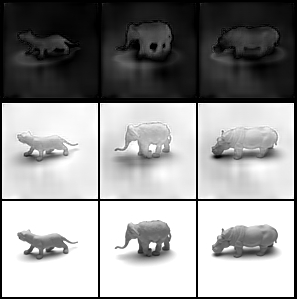
\includegraphics[width=1.0\columnwidth]{./assets/128sampleGANComparison_75_26.png}
\caption{Bottom: 128 sample Mitsuba passed into GAN, Middle: Output of refiner.  Top: Absolute value difference between full sample the rendered image and the refined image. This particular GAN seems to have brightened up the object albedo and dramatically expanded the shadows.  The performance of using the output from this refiner was 75.26\%. and training directly off of the 128 sample target achieved 74.84\%.}
\label{fig:GAN_128}
\end{figure}

\begin{figure}[h!]
\centering
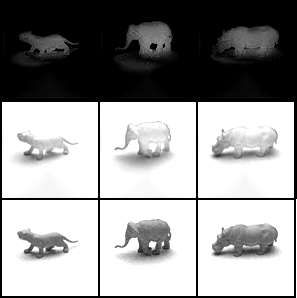
\includegraphics[width=1.0\columnwidth]{./assets/4sampleGANComparison_77_65.png}
\caption{Bottom: 4 sample Mitsuba image passed into GAN, Middle: Output of refiner.  Top: Absolute value difference between the full sample rendered image and the refined image. This particular GAN seems to have brightened up the object albedo, denoised it, lightend it and expanded the shadows to the left.  The performance of using the output from this refiner was 77.65\%. and training directly off of the 4 sample target achieved 72.89\%.  Training off the denoised image achieved 73.56\%.}
\label{fig:GAN_4}
\end{figure}

\begin{figure}[h!]
\centering
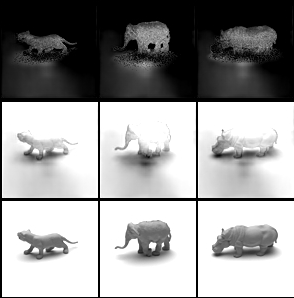
\includegraphics[width=1.0\columnwidth]{./assets/1sampleGANComparison_72_84.png}
\caption{Bottom: 1 sample Mitsuba image passed into GAN, Middle: Output of refiner.  Top: Absolute value difference between the full sampled rendered image and the refined image. This particular GAN seems to have brightened up the object albedo so much that it erased the top parts of the objects. It has denoised it and has darkened and expanded the shadows down and to the left.  The performance of using the output from this refiner was 72.84\%. and training directly off of the 1 sample target achieved 57.21\%.  Training off the denoised image achieved 71.48\%.}
\label{fig:GAN_1}
\end{figure}
1 sample input GANs scored 72.84\% versus 71.48\% for denoising the same image. See figure \ref{fig:GAN_1} for more details.  The accuracy of the best 4 sample input GAN was 77.65\% versus 73.56\% when just denoised. This was the biggest improvement the GANs achieved versus denoising. See figure \ref{fig:GAN_4} for more details.  With the 128 sample input GAN the performance improved to 75.26\% from 74.84\%. See figure \ref{fig:GAN_128} for more details. \\

\subsubsection{Training using multiple GANs} \label{sec:multigans}

The next experiment is a little different from the rest, as we use more training data and is therefore not quite as comparable.  However, the amount of training data which that would have to be generated in a GI renderer remains the same.  The major change is that we use the GAN models from the top ten ranked epochs to create their own refined version of the data.\\

The new dataset is an aggregation of the different refined datasets.  The costly pre-rendering of the input images is not changed and the run-time rendering refinement is longer but insignificant compared to GI rendering time.  In our experiments, it took a minute longer to generate 10 times as much data by running the dataset through ten GANS on an NVIDIA Titan X Maxwell GPU. %Even better, the GANs are already there from the training phase and the ranking is already being done. 
The added time for using this method is negligible except for extra time required to train on a larger dataset.\\

The resulting performance was significantly better than the best quality GI render, denoising or single GAN output.  The best multi-GAN performance for 1-sample data was 85.23\% using 4 GANs.  For 4-sample data, the best performance came from using 7 GANs and scored 84.37\%. This is close to reducing the error between the best GI rendering and real data by half. Using 128-samples data 7 GANs scored 87.33\%. This reduced the difference between training on real data and the best rendering method by more than half!\\ 

In other words, using 128-sample GI rendering is 78.77\% as effective as using real data\footnote{74.84 is 78.77\% of 95.01}.  When you use this measure, a single GAN can boost the effectiveness of synthetic data to 80.01\% of real data.  When an ensemble of GANS is used the synthetic data generated is 91.92\% as effective as real data. 
\\

%We have found that you can use a lower sample count image and boost it with a the byproducts of GAN training and reduce the gap between the most realistic rendering methods and real data by half, and slightly more so if you use a high sample count render.  Furthermore, because it is using the byproducts of normal GAN training, it is not more expensive to create the models for this method. The differences in computation are the up front dataset generation from the output of multiple GAN models and having to train on a larger dataset.\\

It is easy to see why this method works. We are creating a more diverse training dataset that has already been tested to be close to the domain of the real dataset.  However, there are diminishing returns.  Adding any more than 8 GANS did not result in better performance.  That may have to do with having a highly weighted regularization loss which prevented the GAN's refined images from deviating too far from the original rendering.  



%%%%%%%%%%%%%%%%%%%%%%%%%%%%%%%%%%%%%%%%%%%%%%%%%%%%%%%%%%%%%%%%%%%%%%%%%%%%%%%%%%%%%%%%%%%%%%%%%%%%%%%%%%%%
%%%%%%%%%%%%%%%%%%%%%%%%%%%%%%%%%%%%%%%%%%%%%%%%%%%%%%%%%%%%%%%%%%%%%%%%%%%%%%%%%%%%%%%%%%%%%%%%%%%%%%%%%%%%
\section{Conclusion and Future Work}
\subsection{Conclusion}

By using a special dataset consisting of the same scene in both synthetic and real images, we have been able to directly compare different image synthesis techniques and isolate performance differences due to shading.  We have shown that diffuse shading alone doesn't do much better than just using a silhouette, and shadows are important and outperform diffuse shading.  Most importantly, we have shown ways to approximate the effectiveness of the best GI rendering method and how to beat it,  and how to approximate full sample GI while using less computation. Furthermore, we have also shown that by using multiple GAN models you can beat GI simulation by a significant margin and approach the performance of using real data. 

\subsection{Future Work}

Because the multiple GAN training model has shown the most promise, an interesting area to research next would be to predict ensembles able produce the best datasets before going through the trouble of training them.
In the future, we intend to expand the dataset by re-photographing the objects and capturing a light probe.  That way, we can eliminate the difference in lighting conditions between the real and the fake images and allow the performance of different shading methods to be more accurately measured.
\begin{comment}
\begin{itemize}
\item  Learn lighting in real data using SH network and using unsupervised adversarial training with unlabeled real images... with a single lighting condition.
\item Do 2 bounce lighting training but composite AO.  This is closer to modern game engines that calculate SSAO.
\item Do 3 bounce lighting. Some game engines can do an extra bounce.  Also cheaper.  (NEW PAPER/OR CATEGORY IN THIS PAPER: Take 2 and 3 bounce pairs and learn the 3rd bounce)
\item Do GAN on 2 bounce and 3 bounce lighting to see if it gets near the more expensive methods.
\end{itemize}
\end{comment}
\begin{comment}
\begin{table}[]
\centering
\label{tblallrefined}
\begin{tabular}{|l|r|r|r|r|}
\hline
\multicolumn{1}{|c|}{\textbf{Input}} & \multicolumn{1}{c|}{\textbf{1 Sample}} & \multicolumn{1}{c|}{\textbf{4 Samples}} & \multicolumn{1}{c|}{\textbf{128 Samples}} & \multicolumn{1}{c|}{\textbf{A.O.}} \\ \hline
Mitsuba Output Image                 & 57.21\%                                & 72.89\%                                 & 74.84\%                                   & 58.25\%                                \\
Denoised Images                     & 71.48\%                                & 73.56\%                                 & N/A                                       & N/A                                \\
Single GAN Output                     & 59.20\%                                & 70.40\%                                 & 76.09\%                                   & 63.51\%                            \\
Multiple GAN Output                  & 78.94\%                                   & 84.37\%                                 & 85.33\%                                   & 74.49\%                            \\ \hline
\multicolumn{5}{|c|}{\textbf{Performance of GI Rendered Refined Images}}                                                                                                                                             \\ \hline
\end{tabular}
\caption{Comparison of GI Rendered Refined Image Performance. AO images are actually the g-buffer occlusion channel multiplied by the g-buffer albedo channel.  The GAN output refers to if only one GAN was used to refine the dataset or if the dataset was expanded by multiple GANs each refining their own copy and then combining them into one larger dataset.  See section \ref{sec:gans} for further details.}
\end{table}

\begin{table}[]
\centering
\label{tblnonGI}
\begin{tabular}{|l|r|}
\hline
\multicolumn{1}{|c|}{\textbf{Input}} & \multicolumn{1}{c|}{\textbf{Accuracy}} \\ \hline
Albedo Only                          & 46.20\%                                \\
Learned SH Shading                   & 48.52\%                                \\
SH Shading + AO                      & 55.80\%                                \\
Shadow Mapped (2 Bounce)              & 55.78\%                                \\ 
\textbf{Real Images}                           & \textbf{95.01}\%                                \\ \hline
\multicolumn{2}{|c|}{\textbf{Performance Of Non GI Rendering}}                \\ \hline
\end{tabular}
\caption{Non Global Illumination Based Rendering Performance. Albedo Only is passing in the albedo map see figure \ref{fig:GBUFFER_ALBEDO}. Learned SH Shading is unshadowed shading and SH Shading + AO is unshadowed shading with the g-buffer occlusion channel multiplied against the result. See section \ref{sec:learned_sh} for more detail. Shadow Mapped (2 Bounce) is a shading plus shadowing that is described in section \ref{sec:2bounce}. } 
\end{table}


\subsection{Ambient Occlusion Conclusions}
\subsubsection{Varying Lighting}
Learning Spherical Harmonics certainly works for a single lighting condition.  But a problem we forsee is that the test data is under six different lighting conditions and we might want to learn either multiple lighting conditions or have the network be able to learn an arbitrary number of lighting conditions (no design limit to the number of lighting conditions).  

How do we do this?  Is there a way to have feature map count like convolutions?  Like input of 1x96x96 and output Nx1x96x96?  I think this might work.
\subsubsection{Learning Albedo}
During initial experiments we noticed that if the object albedo was not close the non GAN (we didn't have GANs implemented yet) networks would not do better than random guessing on the test set.  However once albedo was approximately the same (in our particular case a medium gray) test performance shot up.  Therefore, it was decided that albedo should be a learnable parameter so object color could be optimized for learning.

The question that arises is should albedo be per object, per material or per pixel?  We will have to try all three.  My guess per object and per material will the most interpretable but per pixel might be the best(or might overfit quickly).

\subsubsection{Shadows and Ambient Occlusion}
While exploring ambient occlusion based images for training we noticed that objects that had minimal shadow, such as people, cars and trucks, in the real data classified well when using AO images.  People objects have the toy base which mostly covers the shadow and cars are low enough to the ground that the shadow doesn't take a large percentage of the image.  However the objects that cast relatively large shadows such as animals an planes have very poor performance when training with AO rendered images.  Shadows Matter!\\

See Figures \ref{fig:mitsuba-AO} and \ref{fig:mitsuba-AO2} for sample renders.

\end{comment}
\begin{comment}
%Connor says that this was on training data that wasn't centered and put into an 80x80 box
\begin{lstlisting}[language=bash]
%python2 main.py --viz-data --use-visdom --visdom-url=http://172.24.70.20 --visdom-port=8097 --train-type=mcmitsuba --data-dir=datasets/mitsuba/large/path/ --lr=1e-5 --epochs=100
%
^^^^^^^^^^^^^^^^^^^^^^^^^^^^^^^^^^^^^^^^^^^^^^^^^^^^^^^^^^^^^^^^^^^^^^^
^^^^^^^^^^^^^^^^^^^^^^^^^^^^^^^^^^^^^^^^^^^^^^^^^^^^^^^^^^^^^^^^^^^^^^^
Best accuracy was 53.63% in epoch 86
ConfusionMatrix:
[[      73     131     509       4      93]   9.012%	[class: animal]
 [       0     585     225       0       0]   72.222%	[class: people]
 [       9       1     542      51     207]   66.914%	[class: plane]
 [      46      14      96     544     110]   67.160%	[class: truck]
 [      61       5     180     136     428]]  52.840%	[class: car]
 + average row correct: 53.63
 + average rowUcol correct (VOC measure): 37.59%
 + global correct: 53.63%
^^^^^^^^^^^^^^^^^^^^^^^^^^^^^^^^^^^^^^^^^^^^^^^^^^^^^^^^^^^^^^^^^^^^^^^
^^^^^^^^^^^^^^^^^^^^^^^^^^^^^^^^^^^^^^^^^^^^^^^^^^^^^^^^^^^^^^^^^^^^^^^
\end{lstlisting}

\begin{figure}[h!]
\centering
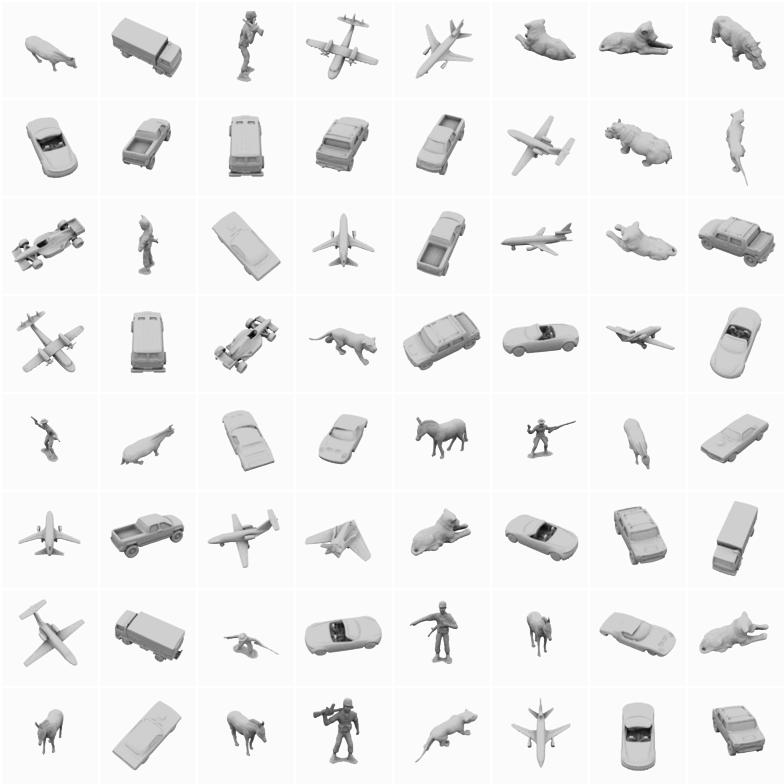
\includegraphics[width=0.8\textwidth]{./assets/mcm-train.png}
\caption{A sample of some of the images generated with Mitsuba using an Ambient Occlusion rendering technique but with a scene lacking a ground plane.}
\label{fig:mitsuba-AO-no-ground}
\end{figure}

In our test we tried using AO to simulate shadows with a relatively short ray length versus a longer ray length.  The difference is that the occlusion calculated was more local and better suited for the environment the test data was photographed in.  We note that here, not only was the accuracy higher than the previous test, but the difference between the highest accuracy label and the lowest accuracy label is much smaller.  The long ray length AO training data only produced a classifier with about 53\% accuracy versus 63\% for a shorter length.  The is approximately the difference between OpenGL and GAN learned shading.  This makes sense in that long ray AO produced a mismatch in the lighting from the test set just like the directional lighting in the OpenGL set.  The shorter ray AO as well as the GAN softened the shadowing which is closer to the test data and as a result they both performed better.\\

%%%%%%%%%%%%%%%%%%%%%%%%%%%%%%%%%%%%%%%%%%%%%%%%%%%%%%%%%%%%%%%%%%%%%%%%%%%%%%%%%%%%%%%%%%%%%%%%%%%%%%%%%%%%
\subsection{Computational Cost}
%%%%%%%%%%%%%%%%%%%%%%%%%%%%%%%%%%%%%%%%%%%%%%%%%%%%%%%%%%%%%%%%%%%%%%%%%%%%%%%%%%%%%%%%%%%%%%%%%%%%%%%%%%%%

Calculating AO properly is expensive and required a global-illumination renderer to sample at the geometry surface and fire rays sampling the hemisphere for any intersections with solid surfaces. However there are techniques that you can use a GPU to approximate AO in real-time.  However the effect of this approximation should be measured.  This is future work.

\end{comment}
\begin{comment}
\begin{lstlisting}[language=bash]
python2 main.py --viz-data --use-visdom --visdom-url=http://172.24.70.20 --visdom-port=8097 --train-type=mcmitsuba --data-dir=datasets/mitsuba/large/path/ --lr=1e-3 --epochs=300 --add-noise

^^^^^^^^^^^^^^^^^^^^^^^^^^^^^^^^^^^^^^^^^^^^^^^^^^^^^^^^^^^^^^^^^^^^^^^
^^^^^^^^^^^^^^^^^^^^^^^^^^^^^^^^^^^^^^^^^^^^^^^^^^^^^^^^^^^^^^^^^^^^^^^
Best accuracy was 63.06% in epoch 141
ConfusionMatrix:
[[     377     218     151      11      53]   46.543%	[class: animal]
 [       7     652     121      12      18]   80.494%	[class: people]
 [      91      31     632      36      20]   78.025%	[class: plane]
 [      96      59      27     535      93]   66.049%	[class: truck]
 [     223      48      20     161     358]]  44.198%	[class: car]
 + average row correct: 63.06
 + average rowUcol correct (VOC measure): 46.12%
 + global correct: 63.06%
^^^^^^^^^^^^^^^^^^^^^^^^^^^^^^^^^^^^^^^^^^^^^^^^^^^^^^^^^^^^^^^^^^^^^^^
^^^^^^^^^^^^^^^^^^^^^^^^^^^^^^^^^^^^^^^^^^^^^^^^^^^^^^^^^^^^^^^^^^^^^^^

\end{lstlisting}

\begin{figure}[h!]
\centering
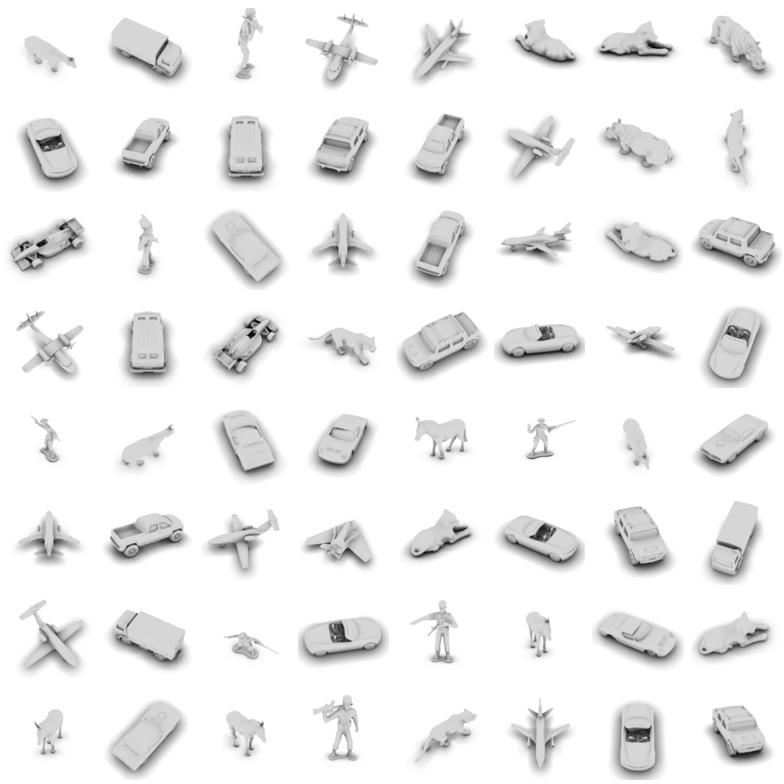
\includegraphics[width=0.8\textwidth]{./assets/mcm-train2.png}
\caption{A sample of some of the images generated with Mitsuba using an Ambient Occlusion rendering technique. Here, a ground plane was introduced to create shadow and the AO ray length was reduced.}
\label{fig:mitsuba-AO2}
\end{figure}
\end{comment}

%%%%%%%%%%%%%%%%%%%%%%%%%%%%%%%%%%%%%%%%%%%%%%%%%%%%%%%%%%%%%%%%%%%%%%%%%%%%%%%%%%%%%%%%%%%%%%%%%%%%%%%%%%%%
%%%%%%%%%%%%%%%%%%%%%%%%%%%%%%%%%%%%%%%%%%%%%%%%%%%%%%%%%%%%%%%%%%%%%%%%%%%%%%%%%%%%%%%%%%%%%%%%%%%%%%%%%%%%

\newpage



%%%%%%%%%%%%%%%%%%%%%%%%%%%%%%%%%%%%%%%%%%%%%%%%%%%%%%%%%%%%%%%%%%%%%%%%%%%%%%%%%%%%%%%%%%%%%%%%%%%%%%%%%%%%
%%%%%%%%%%%%%%%%%%%%%%%%%%%%%%%%%%%%%%%%%%%%%%%%%%%%%%%%%%%%%%%%%%%%%%%%%%%%%%%%%%%%%%%%%%%%%%%%%%%%%%%%%%%%
%%%%%%%%%%%%%%%%%%%%%%%%%%%%%%%%%%%%%%%%%%%%%%%%%%%%%%%%%%%%%%%%%%%%%%%%%%%%%%%%%%%%%%%%%%%%%%%%%%%%%%%%%%%%
%%%%%%%%%%%%%%%%%%%%%%%%%%%%%%%%%%%%%%%%%%%%%%%%%%%%%%%%%%%%%%%%%%%%%%%%%%%%%%%%%%%%%%%%%%%%%%%%%%%%%%%%%%%%
%%%%%%%%%%%%%%%%%%%%%%%%%%%%%%%%%%%%%%%%%%%%%%%%%%%%%%%%%%%%%%%%%%%%%%%%%%%%%%%%%%%%%%%%%%%%%%%%%%%%%%%%%%%%
%%%%%%%%%%%%%%%%%%%%%%%%%%%%%%%%%%%%%%%%%%%%%%%%%%%%%%%%%%%%%%%%%%%%%%%%%%%%%%%%%%%%%%%%%%%%%%%%%%%%%%%%%%%%
%%%%%%%%%%%%%%%%%%%%%%%%%%%%%%%%%%%%%%%%%%%%%%%%%%%%%%%%%%%%%%%%%%%%%%%%%%%%%%%%%%%%%%%%%%%%%%%%%%%%%%%%%%%%
%%%%%%%%%%%%%%%%%%%%%%%%%%%%%%%%%%%%%%%%%%%%%%%%%%%%%%%%%%%%%%%%%%%%%%%%%%%%%%%%%%%%%%%%%%%%%%%%%%%%%%%%%%%%
%%%%%%%%%%%%%%%%%%%%%%%%%%%%%%%%%%%%%%%%%%%%%%%%%%%%%%%%%%%%%%%%%%%%%%%%%%%%%%%%%%%%%%%%%%%%%%%%%%%%%%%%%%%%
%%%%%%%%%%%%%%%%%%%%%%%%%%%%%%%%%%%%%%%%%%%%%%%%%%%%%%%%%%%%%%%%%%%%%%%%%%%%%%%%%%%%%%%%%%%%%%%%%%%%%%%%%%%%
%%%%%%%%%%%%%%%%%%%%%%%%%%%%%%%%%%%%%%%%%%%%%%%%%%%%%%%%%%%%%%%%%%%%%%%%%%%%%%%%%%%%%%%%%%%%%%%%%%%%%%%%%%%%
%%%%%%%%%%%%%%%%%%%%%%%%%%%%%%%%%%%%%%%%%%%%%%%%%%%%%%%%%%%%%%%%%%%%%%%%%%%%%%%%%%%%%%%%%%%%%%%%%%%%%%%%%%%%
%%%%%%%%%%%%%%%%%%%%%%%%%%%%%%%%%%%%%%%%%%%%%%%%%%%%%%%%%%%%%%%%%%%%%%%%%%%%%%%%%%%%%%%%%%%%%%%%%%%%%%%%%%%%
%%%%%%%%%%%%%%%%%%%%%%%%%%%%%%%%%%%%%%%%%%%%%%%%%%%%%%%%%%%%%%%%%%%%%%%%%%%%%%%%%%%%%%%%%%%%%%%%%%%%%%%%%%%%
%%%%%%%%%%%%%%%%%%%%%%%%%%%%%%%%%%%%%%%%%%%%%%%%%%%%%%%%%%%%%%%%%%%%%%%%%%%%%%%%%%%%%%%%%%%%%%%%%%%%%%%%%%%%

\begin{comment}
\section{APPENDIX A - Non-Standard G-Buffer Experiments}
\subsection{Randomized SH Weights Experiment}
The following experiments train a classifier with a generative SH net but this time the loss ignored and the generative net has its parameters randomly set from a uniform distribution.
The classifier is effectively trained with randomly lit objects. Where the lighting is restricted to a smooth function along a sphere's surface.
\begin{enumerate}
\item Per Training Epoch
\begin{enumerate}
\item Randomly set SH weights
\item Iterate through all of the training data which in this case is the normal buffer part of a G-Buffer 
\item Classify generated images.
\item Use loss to update the classifier.
\end{enumerate}
\end{enumerate}

Then use the trained classifier C to classify real test images.\\
Results for 500 epochs
\begin{lstlisting}[language=bash]
%$ python test_sh4_use_random_weights.py --viz-data --visdom-env kris 
%--use-visdom --epochs 500 --lr 1e-3 --data-dir datasets/opengl/small/ --cuda-device 1
%# Using random weights for SH to train classifier.  500 epochs. 
^^^^^^^^^^^^^^^^^^^^^^^^^^^^^^^^^^^^^^^^^^^^^^^^^^^^^^^^^^^^^^^^^^^^^^^
^^^^^^^^^^^^^^^^^^^^^^^^^^^^^^^^^^^^^^^^^^^^^^^^^^^^^^^^^^^^^^^^^^^^^^^
Best accuracy was 46.86% in epoch 424
ConfusionMatrix:
[[     414      92     278      18       8]   51.111%	[class: animal]
 [      39     760      11       0       0]   93.827%	[class: people]
 [      78     110     618       1       3]   76.296%	[class: plane]
 [     160       8     497      18     127]   2.222%	[class: truck]
 [     240       5     463      14      88]]  10.864%	[class: car]
 + average row correct: 46.86
 + average rowUcol correct (VOC measure): 29.36%
 + global correct: 46.86%
^^^^^^^^^^^^^^^^^^^^^^^^^^^^^^^^^^^^^^^^^^^^^^^^^^^^^^^^^^^^^^^^^^^^^^^
^^^^^^^^^^^^^^^^^^^^^^^^^^^^^^^^^^^^^^^^^^^^^^^^^^^^^^^^^^^^^^^^^^^^^^^
\end{lstlisting}
Results for 10,000 epochs
\begin{lstlisting}[language=bash]

%$ python test_sh4_use_random_weights.py --epochs 10000 --lr 1e-3 
%--data-dir datasets/opengl/small/
%# trained with random sh weights per epoch. No loss used to guide it.
^^^^^^^^^^^^^^^^^^^^^^^^^^^^^^^^^^^^^^^^^^^^^^^^^^^^^^^^^^^^^^^^^^^^^^^
^^^^^^^^^^^^^^^^^^^^^^^^^^^^^^^^^^^^^^^^^^^^^^^^^^^^^^^^^^^^^^^^^^^^^^^
Best accuracy was 47.78% in epoch 646
ConfusionMatrix:
[[     554     117      92      47       0]   68.395%   [class: animal]
 [      26     762      13       9       0]   94.074%   [class: people]
 [     205     177     415      13       0]   51.235%   [class: plane]
 [     221       5     373     190      21]   23.457%   [class: truck]
 [     319       7     307     163      14]]  1.728%    [class: car]
 + average row correct: 47.78
 + average rowUcol correct (VOC measure): 29.85%
 + global correct: 47.78%
^^^^^^^^^^^^^^^^^^^^^^^^^^^^^^^^^^^^^^^^^^^^^^^^^^^^^^^^^^^^^^^^^^^^^^^
^^^^^^^^^^^^^^^^^^^^^^^^^^^^^^^^^^^^^^^^^^^^^^^^^^^^^^^^^^^^^^^^^^^^^^^
\end{lstlisting}
Results for 100,000 epochs
\begin{lstlisting}[language=bash]
%$ python test_sh4_use_random_weights.py --epochs 100000 --lr 1e-3 
%--data-dir datasets/opengl/small/ 
%# trained with random sh weights per epoch. No loss used to guide it.
^^^^^^^^^^^^^^^^^^^^^^^^^^^^^^^^^^^^^^^^^^^^^^^^^^^^^^^^^^^^^^^^^^^^^^^
^^^^^^^^^^^^^^^^^^^^^^^^^^^^^^^^^^^^^^^^^^^^^^^^^^^^^^^^^^^^^^^^^^^^^^^
Best accuracy was 49.43% in epoch 1660
ConfusionMatrix:
[[     355      74     271       2     108]   43.827%   [class: animal]
 [      40     717      50       3       0]   88.519%   [class: people]
 [      57      57     601       1      94]   74.198%   [class: plane]
 [      28       0     319      36     427]   4.444%    [class: truck]
 [      53       0     427      37     293]]  36.173%   [class: car]
 + average row correct: 49.43
 + average rowUcol correct (VOC measure): 33.75%
 + global correct: 49.43%
^^^^^^^^^^^^^^^^^^^^^^^^^^^^^^^^^^^^^^^^^^^^^^^^^^^^^^^^^^^^^^^^^^^^^^^
^^^^^^^^^^^^^^^^^^^^^^^^^^^^^^^^^^^^^^^^^^^^^^^^^^^^^^^^^^^^^^^^^^^^^^^
\end{lstlisting}
As you can see the more examples it is shown the better it gets however there are clearly diminishing returns and it seems that it didn't benefit from more than 20,000 epochs so adding any epochs would probably gain nothing in accuracy.
\subsection{Basic OpenGL Directional Lighting and Shadow Mapping}
\begin{figure}[h!]
\centering
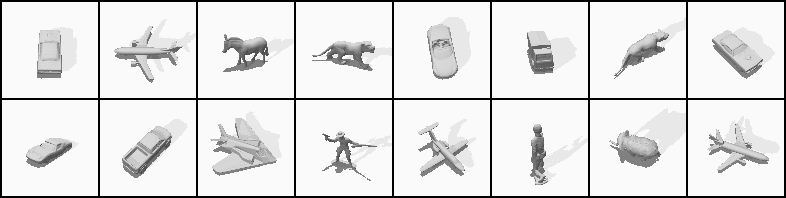
\includegraphics[width=0.95\textwidth]{./assets/dotsynthshadow_training.jpg}
\caption{OpenGL Rendering Example.  Notice the two shadows with varying intensity.}
\label{fig:OGLDOTSYNTH}
\end{figure}
\begin{figure}[h!]
\centering
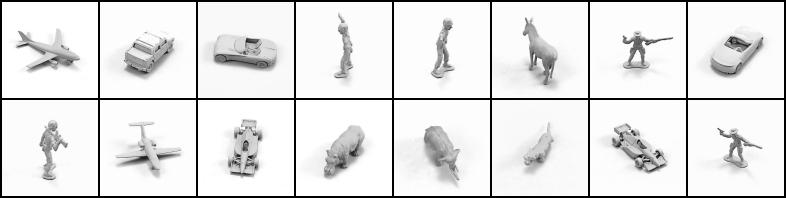
\includegraphics[width=0.95\textwidth]{./assets/TrainDataReal16.png}
\caption{Real NORB Training Data Photographs}
\label{fig:REALTRAIN}
\end{figure}
The most basic rendering was with a simple OpenGL based renderer that had two directional lights of differing intensities.  Shadows were calculated per light.  See Figure \ref{fig:OGLDOTSYNTH} for an example rendering of some training data. Compare it with real training data in Figure \ref{fig:REALTRAIN}.\\
The OpenGL API makes this kind of rendering very efficient on a GPU and thousands of images can be generated per second.  The images created for this test took less than a millisecond to calculate.  The copy down to the CPU and writing to disk slowed everything down to roughly 300 images a second rendered and written to disk on a Titan X (Maxwell). If buffers were shared with CUDA then used directly in training the rendering time would be insignificant.  Because this is the easiest and cheapest method for creating data we will consider it the baseline for comparing the rest of the rendering methods.\\
While this method is cheap it is also not very effective in training a classifier.  See Figure \ref{fig:PLOTOPENGL} to see that we only get around 50\% accuracy when testing on the real NORB test data.
\begin{figure}[h!]
\centering
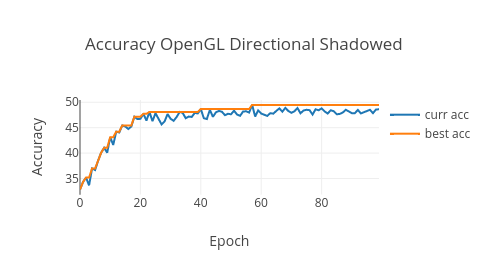
\includegraphics[width=0.95\textwidth]{./assets/OpenGL_DotSynth_Performance.png}
\caption{Accuracy of classifier trained with OpenGL Directional Lighting with Shadows.  It maxed out at 49.48\%.}
\label{fig:PLOTOPENGL}
\end{figure}

\end{comment}
%\begin{lstlisting}[language=bash]
%^^^^^^^^^^^^^^^^^^^^^^^^^^^^^^^^^^^^^^^^^^^^^^^^^^^^^^^^^^^^^^^^^^^^^^^
%^^^^^^^^^^^^^^^^^^^^^^^^^^^^^^^^^^^^^^^^^^^^^^^^^^^^^^^^^^^^^^^^^^^^^^^
%Best accuracy was 49.48% in epoch 58
%ConfusionMatrix:
%[[     685       0       0       9     116]   84.568%	[class: animal]
% [     135     321       0       0     354]   39.630%	[class: people]
% [     354      14       0      28     414]   0.000%	[class: plane]
% [     116       0       0     401     293]   49.506%	[class: truck]
% [     183       0      20      10     597]]  73.704%	[class: car]
% + average row correct: 49.48
% + average rowUcol correct (VOC measure): 31.73%
% + global correct: 49.48%
%^^^^^^^^^^^^^^^^^^^^^^^^^^^^^^^^^^^^^^^^^^^^^^^^^^^^^^^^^^^^^^^^^^^^^^^
%^^^^^^^^^^^^^^^^^^^^^^^^^^^^^^^^^^^^^^^^^^^^^^^^^^^^^^^^^^^^^^^^^^^^^^^
%\end{lstlisting}
%
%\subsection{Training with Global Illumination Renderer}
%The following experiments were conducted using images calculated using Mitsuba with various integrators, such as Direct (Ray Tracing) and Path (Path Tracing).
%\begin{lstlisting}[language=bash]
%$ python main.py --train-type 'trainsynth' --lr 1e-4
%# This is on 48600 direct integrator mitsuba.  10 lighting conditions and 
%# only 1 test lighting condition
%^^^^^^^^^^^^^^^^^^^^^^^^^^^^^^^^^^^^^^^^^^^^^^^^^^^^^^^^^^^^^^^^^^^^^^^
%ConfusionMatrix:
%[[     700      46       7       0      57]   86.420%	[class: animal]
% [       5     724      71       0      10]   89.383%	[class: people]
% [      57       6     704       0      43]   86.914%	[class: plane]
% [      44       0       0     734      32]   90.617%	[class: truck]
% [      16       2      39     401     352]]  43.457%	[class: car]
% + average row correct: 79.36
% + average rowUcol correct (VOC measure): 66.49%
% + global correct: 79.36%
%-----> *** Best model so far.  Saving checkpoint for epoch 28 pct 79.36*** <----
%^^^^^^^^^^^^^^^^^^^^^^^^^^^^^^^^^^^^^^^^^^^^^^^^^^^^^^^^^^^^^^^^^^^^^^^
%
%$ python main.py --train-type 'trainsynth' --lr 5e-6 
%--data-dir datasets/mitsuba/large/path/ --epochs 300
%# This is on 48600 path integrator mitsuba.  10 lighting conditions and only 1 
%# test lighting condition
%^^^^^^^^^^^^^^^^^^^^^^^^^^^^^^^^^^^^^^^^^^^^^^^^^^^^^^^^^^^^^^^^^^^^^^^
%Best accuracy was 74.96% in epoch 169
%ConfusionMatrix:
%[[     616     104      58       0      32]   76.049%   [class: animal]
% [       2     684     124       0       0]   84.444%   [class: people]
% [      10       4     708       8      80]   87.407%   [class: plane]
% [      76       0       8     647      79]   79.877%   [class: truck]
% [     110       0      45     274     381]]  47.037%   [class: car]
% + average row correct: 74.96
% + average rowUcol correct (VOC measure): 60.14%
% + global correct: 74.96%
% 
%$ python main.py --train-type 'genbprop' --lr 1e-4 --epochs 300 --viz-data
%# This is on 51,839 gbuffer(normals).  Test set is 12,960 gbuffer images.  
%# The pretrained model had 90.79% accuracy on real data and was trained from real data.
%^^^^^^^^^^^^^^^^^^^^^^^^^^^^^^^^^^^^^^^^^^^^^^^^^^^^^^^^^^^^^^^^^^^^^^^
%^^^^^^^^^^^^^^^^^^^^^^^^^^^^^^^^^^^^^^^^^^^^^^^^^^^^^^^^^^^^^^^^^^^^^^^
%Best accuracy was 85.06% in epoch 284
%ConfusionMatrix:
%[[    2592       0       0       0       0]   100.000%  [class: animal]
% [       5    2587       0       0       0]   99.807%   [class: people]
% [     161       0    1426      97     908]   55.015%   [class: plane]
% [      16       0       4    2140     432]   82.562%   [class: truck]
% [      14       0      29     270    2279]]  87.924%   [class: car]
% + average row correct: 85.06
% + average rowUcol correct (VOC measure): 75.48%
% + global correct: 85.06%
%^^^^^^^^^^^^^^^^^^^^^^^^^^^^^^^^^^^^^^^^^^^^^^^^^^^^^^^^^^^^^^^^^^^^^^^
%^^^^^^^^^^^^^^^^^^^^^^^^^^^^^^^^^^^^^^^^^^^^^^^^^^^^^^^^^^^^^^^^^^^^^^^
% 
%python main.py --train-type=mcmitsuba --data-dir=datasets/mitsuba/small/path/
%# Trained using combined image, normals, occlusion, and albedo data on 400 synthetic Mitsuba-generated images.
%^^^^^^^^^^^^^^^^^^^^^^^^^^^^^^^^^^^^^^^^^^^^^^^^^^^^^^^^^^^^^^^^^^^^^^^
%^^^^^^^^^^^^^^^^^^^^^^^^^^^^^^^^^^^^^^^^^^^^^^^^^^^^^^^^^^^^^^^^^^^^^^^
%Best accuracy was 74.00% in epoch 49
%ConfusionMatrix:
%[[       8       5       0       7       0]   40.000%	[class: animal]
% [       3      16       0       1       0]   80.000%	[class: people]
% [       1       0      19       0       0]   95.000%	[class: plane]
% [       0       0       2      18       0]   90.000%	[class: truck]
% [       0       0       0       7      13]]  65.000%	[class: car]
% + average row correct: 74.00
% + average rowUcol correct (VOC measure): 60.03%
% + global correct: 74.00%
%^^^^^^^^^^^^^^^^^^^^^^^^^^^^^^^^^^^^^^^^^^^^^^^^^^^^^^^^^^^^^^^^^^^^^^^
%^^^^^^^^^^^^^^^^^^^^^^^^^^^^^^^^^^^^^^^^^^^^^^^^^^^^^^^^^^^^^^^^^^^^^^^
%
% 
%\end{lstlisting}
\begin{comment}
\subsection{Adversarial Training with goal of maximizing classification performance}
G = Generator Network.  Which can be a GBuffer with a Spherical Harmonics or Convolutional Block on top of it.
C = Classifier.  Experiment with architectures.. but start with the one used in the NORB paper.
\subsection{Training method}
G creates rendered synthetic images S.  S is fed into C and C updates its weights but does not send loss to G. After each epoch the real test data S is sent into C and the loss is sent to G to update its weights.  The goal is to only use the misclassification loss to update G.  The goal isn't for G to make images as realistic and as close to S as possible.  Its main goal is to have G produce S that maximizes the performance C learning how to classify R. 

This is a tick - tock pattern where on tick C learns from S and on tock G learns from R fed into C.  Each tick and tock are an "epoch" in the sense that all of the data is passed through once.

\subsection{Adversarial Training using SIMGAN as a baseline}
This has the advantages of being able to use unlabeled data. 
\begin{itemize}
  \item Start with GBuffer.  This might prevent the need for a local adversarial loss.
  \item Also experiment with starting with 
    \begin{itemize}
      \item Directional lighting
      \item AO
      \item Path Traced
      \item Direct Ray Tracing
    \end{itemize}
\end{itemize}
\end{comment}

%
%\subsection{Style Transfer as a data gen technique}
%http://www.creativeai.net/posts/DxEdiP2D74kmkfZrZ/arbitrary-style-transfer-in-real-time-with-adaptive-instance
%
%
%This has the advantage of creating many NPR styles that we can test
%\begin{itemize}
%  \item Start with Pixels of the type:
%    \begin{itemize}
%      \item Directional lighting
%      \item AO
%      \item Path Traced
%      \item Direct Ray Tracing
%    \end{itemize}
%  \item Then use a variety of images to style them and train on them and test performance.
%  \item can we use the loss to update the style????  Maybe. SOMETHING TO TRY.
%  \item this is like a differentiable shader if we can update the style based upon the loss in classification.
%\end{itemize}
%
%\subsection{Train on GBuffer}
%\subsection{Pre-train Classifier on Real Data and make that an adversarial loss for generator}
%\begin{itemize}
%\item What loss should I use to update the generator?
%\item What model should I use for the generator?
%\end{itemize}
%
%\subsection{Learning from Simulated and Unsupervised Images through Adversarial Training}
%For eye gaze tracking they train with synthetic data from the UnityEyes or refined datasets and test on the real data from MPIIGaze.  They don't pre-train of or do any transfer learning.
%\subsection{Experiments}
%\begin{itemize}
%\item Synthetic Data
%\item Synthetic Data x4
%\item Refined Data
%\item Refined Data x4
%\end{itemize}
%
\begin{comment}
\section{APPENDIX B Other Papers}
\subsection{Physically-Based Rendering for Indoor Scene Understanding Using Convolutional Neural Nets}

\subsection{Experiments}
\subsubsection{Terminology}
In the neural network terminology:

\textbf{one epoch} = one forward pass and one backward pass of all the training examples

\textbf{batch size} = the number of training examples in one forward/backward pass. The higher the batch size, the more memory space you'll need.

\textbf{number of iterations} = number of passes, each pass using [batch size] number of examples. To be clear, one pass = one forward pass + one backward pass (we do not count the forward pass and backward pass as two different passes).

Example: if you have 1000 training examples, and your batch size is 500, then it will take 2 iterations to complete 1 epoch.

\subsubsection{Normal Estimation}
Pretraining on synthetic data followed by finetuning on NYUv2 similar to A. Bansal, B.C. Russell, and A. Gupta. "Marr Revisited: 2D-3D alignment via surface normal prediction." CVPR 2016. Using RMSProp they use a learning rate of 1e-3 reducing it by half every 300k iterations for pretraining. (What do they mean by iterations??? It can't be epochs so it must be batches or samples).  For finetuning they use a learning rate of 1e-4 reducing by half every 10k iterations.
\begin{itemize}
\item Model Pretrained on MLT(Path traced metropolis light transport) and finetuned on NYUv2 achieves best performance
\item Model Pretrained on MLT. Compared to training with OpenGLs(2) and trained on NYUv2.
\item MLT indoor and outdoor lighting vs MLT outdoor only. Indoor + Outdoor is better
\end{itemize}

\subsubsection{Semantic Segmentation and Boundary Detection}
Initialize the network with pretrained weights from ImageNet.  Then pretrain on synthetic dataset then finetune on NYUv2. Use SGD with learning rate 1e-5 for pretraining and finetuning.  They say: We also replicate the corresponding state of the art training schedules by pretraining on ImageNet, followed by directly finetuning on NYUv2, for comparison.

The standard SGD is used for optimization. The learning rate is initially set to be smaller (2e-7) to deal with larger image resolution of NYUv2, and is reduced even more, to 1/10 after each 10k iterations on NYUv2(Finetuning). For synthetic data, similar to our procedure in normal estimation the learning rate is reduced every 300k iterations.
\begin{itemize}
\item Model initialized with ImageNet and trained on OpenGL IL.
\item Model initialized with ImageNet and trained on MLT Indoor and Outdoor lighting
\item Model initialized with ImageNet and pretrained on OpenGL IL(Indoor Light), Finetuned on NYUv2
\item Model initialized with ImageNet and pretrained on MLT Indoor and Outdoor lighting, Finetuned on NYUv2
\end{itemize}

\newpage




\begin{lstlisting}[language=bash]
$ python main.py --train-type gansh --viz-data --visdom-env kris
--use-visdom --epochs 300 --lr 1e-3
# this is training off of 239 synthetic training images and testing on one
# lighting condition of real norb (4050 images)
-- THIS CODE IS NOW IN THE BRANCH 'curious_result'
^^^^^^^^^^^^^^^^^^^^^^^^^^^^^^^^^^^^^^^^^^^^^^^^^^^^^^^^^^^^^^^^^^^^^^^
^^^^^^^^^^^^^^^^^^^^^^^^^^^^^^^^^^^^^^^^^^^^^^^^^^^^^^^^^^^^^^^^^^^^^^^
Best accuracy was 92.27% in epoch 145
ConfusionMatrix:
[[     728      35      32       0      15]   89.877%	[class: animal]
 [       2     808       0       0       0]   99.753%	[class: people]
 [      71       0     727       4       8]   89.753%	[class: plane]
 [       3       0       1     757      49]   93.457%	[class: truck]
 [      47       0       0      46     717]]  88.519%	[class: car]
 + average row correct: 92.27
 + average rowUcol correct (VOC measure): 85.84%
 + global correct: 92.27%
^^^^^^^^^^^^^^^^^^^^^^^^^^^^^^^^^^^^^^^^^^^^^^^^^^^^^^^^^^^^^^^^^^^^^^^
^^^^^^^^^^^^^^^^^^^^^^^^^^^^^^^^^^^^^^^^^^^^^^^^^^^^^^^^^^^^^^^^^^^^^^^

$ python main.py --train-type 'trainreal' --lr 1e-4 --visdom-env kris 
--use-visdom --batch-size 128 --lr-drop-width 20 --lr-drop-value 0.85 
--epochs 100
# Trained on single light real data.  Normalized.  Used learning rate 
# schedule that dropped 15% every 20 epochs.
# Used vgg08_bn with linear classifier features at 100.  
^^^^^^^^^^^^^^^^^^^^^^^^^^^^^^^^^^^^^^^^^^^^^^^^^^^^^^^^^^^^^^^^^^^^^^^
^^^^^^^^^^^^^^^^^^^^^^^^^^^^^^^^^^^^^^^^^^^^^^^^^^^^^^^^^^^^^^^^^^^^^^^
Best accuracy was 96.86% in epoch 93
ConfusionMatrix:
[[     782       9       1       0      18]   96.543%	[class: animal]
 [       0     810       0       0       0]   100.000%	[class: people]
 [      22       0     788       0       0]   97.284%	[class: plane]
 [       0       0       0     809       1]   99.877%	[class: truck]
 [       0       0       0      76     734]]  90.617%	[class: car]
 + average row correct: 96.86
 + average rowUcol correct (VOC measure): 93.98%
 + global correct: 96.86%
^^^^^^^^^^^^^^^^^^^^^^^^^^^^^^^^^^^^^^^^^^^^^^^^^^^^^^^^^^^^^^^^^^^^^^^
^^^^^^^^^^^^^^^^^^^^^^^^^^^^^^^^^^^^^^^^^^^^^^^^^^^^^^^^^^^^^^^^^^^^^^^
\subsection{GAN Training}
Inputs to the DeepShading Network are:
\begin{itemize}
\item Normals
\begin{figure}[h!]
\centering
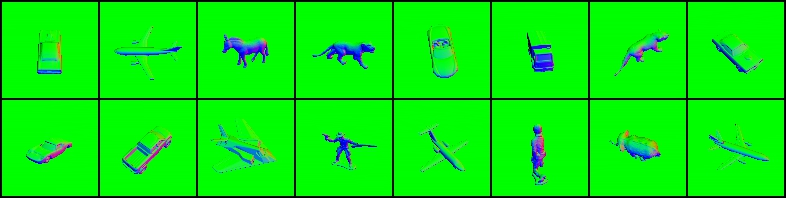
\includegraphics[width=1.0\textwidth]{./assets/synth_world_normals.jpg}
\caption{World Space Normals Map in RGB}
\label{fig:GBUFFER_NORMALS}
\end{figure}

\item Albedo

\begin{figure}[h!]
\centering
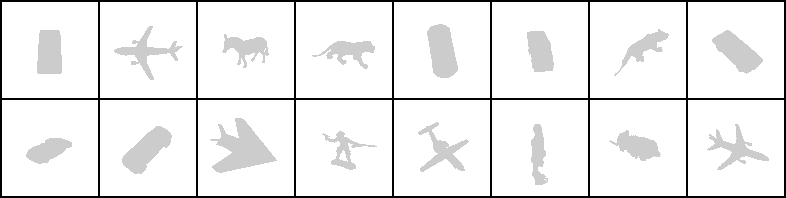
\includegraphics[width=1.0\textwidth]{./assets/synth_albedo.jpg}
\caption{Albedo Map}
\label{fig:GBUFFER_ALBEDO}
\end{figure}

\item Positions

\begin{figure}[h!]
\centering
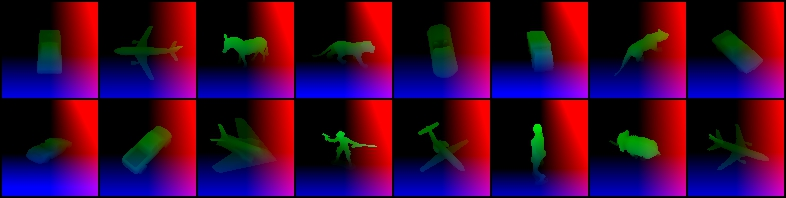
\includegraphics[width=1.0\textwidth]{./assets/synth_world_positions.jpg}
\caption{Albedo Map}
\label{fig:GBUFFER_POSITIONS}
\end{figure}

\item Depth

\begin{figure}[h!]
\centering
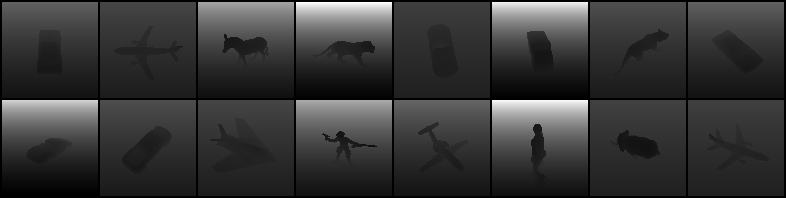
\includegraphics[width=1.0\textwidth]{./assets/synth_linear_depth.jpg}
\caption{Depth Map}
\label{fig:GBUFFER_DEPTH}
\end{figure}

\item Shadow (only one)

\begin{figure}[h!]
\centering
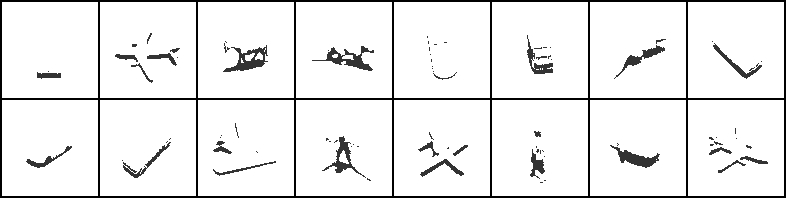
\includegraphics[width=0.8\textwidth]{./assets/synth_occlusion1.jpg}
\caption{Shadow Map}
\label{fig:GBUFFER_SHADOW}
\end{figure}

\begin{figure}[h!]
\centering
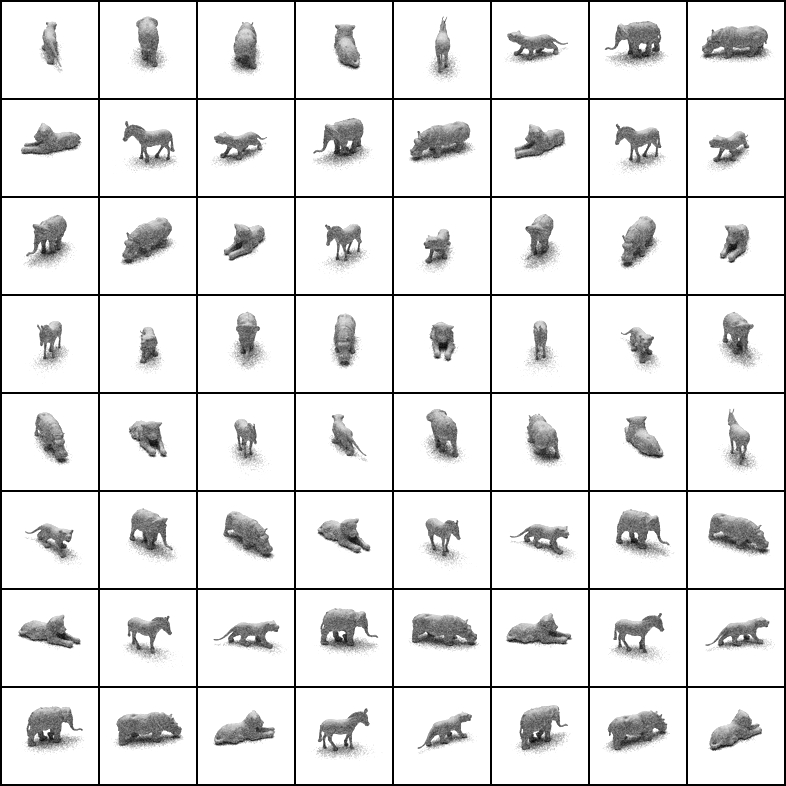
\includegraphics[trim={0 0 392px 687px},clip,width=1.0\textwidth]{./assets/traindata_1_sample.jpg}
\caption{Sample crop 1.}
\label{fig:crop1}
\end{figure}
\begin{figure}[h!]
\centering
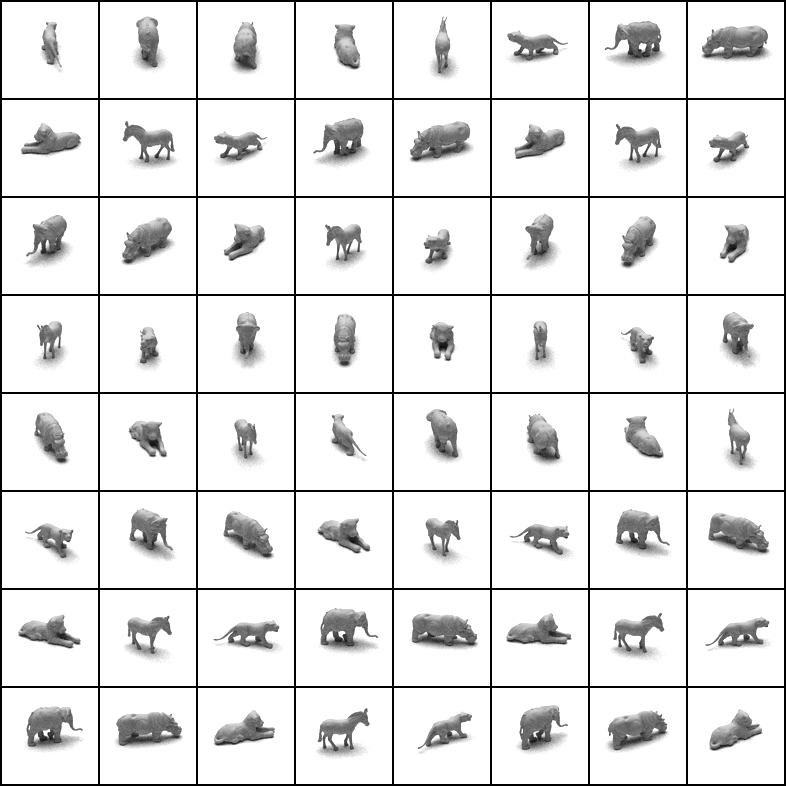
\includegraphics[trim={0 0 392px 687px},clip,width=1.0\textwidth]{./assets/traindata_4_sample.jpg}
\caption{Sample crop 4.}
\label{fig:crop4}
\end{figure}
\begin{figure}[h!]
\centering
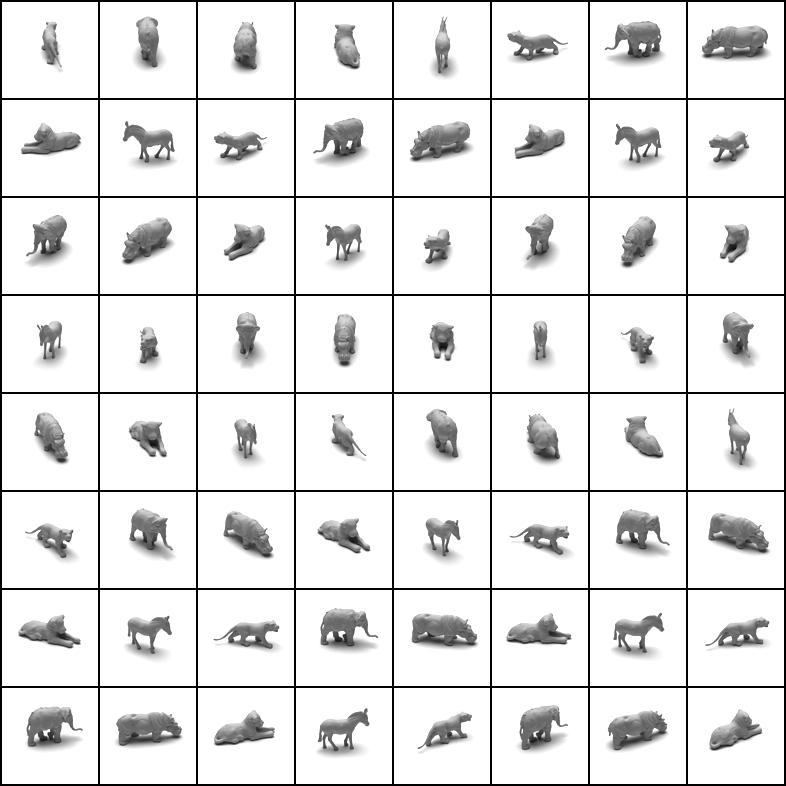
\includegraphics[trim={0 0 392px 687px},clip,width=1.0\textwidth]{./assets/traindata_target_128_sample.jpg}
\caption{Sample crop 128.}
\label{fig:crop128}
\end{figure}

\end{itemize}
\end{comment}

\bibliography{bibliography}{}
\bibliographystyle{plain}
\end{document}
